\documentclass{article}

\usepackage{cancel}
\usepackage{tikz}
\usepackage{amsmath}
\usepackage{geometry}
\usepackage{graphicx}
\usepackage{amsfonts} 
\usepackage{verbatim}
\usepackage{mathrsfs}  
\usepackage{lmodern}
\usepackage{braket}
\usepackage{bookmark}

\hypersetup{
    colorlinks=true,
    linkcolor=black,
}

\renewcommand{\contentsname}{Indice}

\tikzset{block/.style = {draw, fill=white, very thick, rectangle, minimum height=1cm, minimum width=2cm},
         lblock/.style={draw,fill=white,very thick, rectangle, minimum height=3cm, minimum width=1cm},
         sum/.style= {draw, fill=white, very thick, circle, node distance=0.5cm}}

\numberwithin{equation}{subsection}

\title{Appunti di Elettrotecnica ed Elettronica}
\author{Giacomo Sturm}
\date{AA: 2023/2024 - Ing. Informatica}

\begin{document}

\maketitle

\vspace{10mm}

\begin{center}
    Sorgente del file LaTeX disponibile su \url{https://github.com/00Darxk/Elettrotecnica-ed-Elettronica}
\end{center}

\clearpage

\tableofcontents

\clearpage

\section{Nozioni di Base sull'Elettro-Magnetismo}

\subsection{Forza Elettrica}
Le prime analisi documentate sugli effetti elettrici risalgono agli antichi greci, da cui deriva il nome "electron"; $\eta\lambda\varepsilon\kappa\tau\rho o\nu$ in greco. Letteralmente significa ambra, poiché 
quando viene sfregata contro della lana, è capace di attrarre materiali, ovvero è in grado di generare un campo elettrico.

La forza elettrica venne analizzata da Coulomb in maniera simile all'analisi di Newton sulla gravità, poiché le due forze presentano dei comportamenti simili. La forza di 
gravità è una forza attrattiva tra due masse nello spazio, per cui sono presenti due forze applicate ad entrambe le masse di modulo e direzione uguale, ma verso opposto: 
\begin{equation*}
    \vec{F}_{1\to2}=G\displaystyle\frac{m_1m_2}{r^2}\hat{r}_{1\to2}=-\vec{F}_{2\to1}
\end{equation*}
Analogamente la forza elettrica è presente solo nell'interazione tra due elementi dotati di una carica che può presentarsi in due classi diverse, per convezione 
positiva o negativa, vengono misurate in Coulomb $C$ nel SI. Due cariche appartenenti alla stessa classe si oppongono, mentre due cariche appartenenti a due classi diverse 
si attraggono:
\begin{gather}
    \vec{F}_{1\to2}=-k_0\displaystyle\frac{q_1q_2}{r^2}\hat{r}_{1\to2}=-\vec{F}_{2\to1}\\
    F=k_0\displaystyle\frac{|q_1q_2|}{r^2}
\end{gather} 
Viene chiamata $k_0$ costante elettrica nel vuoto. 


La forza di gravità è una forza solamente attrattiva e presenta una sola classe di masse a differenza della forza elettrica. Poiché la forza di gravità si 
presenta solamente dall'interazione tra due masse, una massa singola nello spazio non è soggetta a forze di gravità. Questa massa è pronta ad interagire con un eventuale 
seconda massa per comunicare tra di loro la massa deforma in qualche modo lo spazio. Convenzionalmente si considera una deformazione convessa nella zona di spazio dove 
si trova la massa: 
\begin{center}
    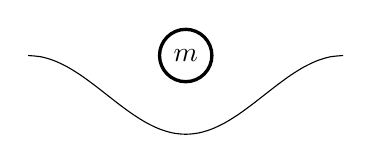
\begin{tikzpicture}[scale=2]
        \node[sum](o)at(0,0){$m$};
        \draw[-]plot[smooth, domain=-1:1](\x,{0.25*cos(180*(\x)-pi r)-0.25});
    \end{tikzpicture}
\end{center}

Poiché le cariche possono appartenere a due classi diverse per convenzione una carica positiva crea una deformazione concava, mentre una negativa una deformarzione convessa: 
\begin{center}
    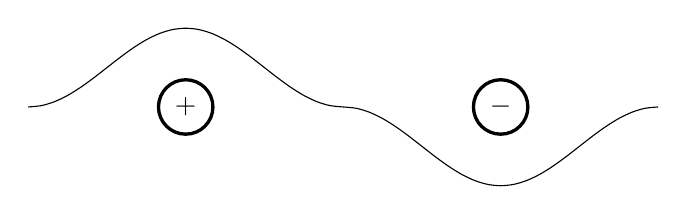
\begin{tikzpicture}[scale=2]
        \node[sum](o1)at(0,0){$+$};
        \draw[-]plot[smooth, domain=-1:1](\x,{-0.25*cos(180*(\x)-pi r)+0.25});
        
        \node[sum](o2)at(2,0){$-$};
        \draw[-]plot[smooth, domain=1:3](\x,{0.25*cos(180*(\x-2)-pi r)-0.25});
    \end{tikzpicture}
\end{center}
Per cui le cariche positive tendono a "scendere", mentre le cariche negative tendono a "salire". La deformazione spaziale è dovuta ad un campo gravitazionale o elettrico, 
dalle interazione del campo si genera una forza gravitazionale o elettrica. 

\subsection{Campo Elettrico}
Un campo elettrico $\vec{E}(x,y,z)$ è un campo vettoriale, ovvero è un insieme di vettori per ogni punto dello spazio dipendenti dalla loro posizione. Per misurare il campo 
generato da una carica $Q$ positiva per convenzione, si considera un'altra carica positiva $q<<Q$ usata per misurare la forza elettrica $\vec{F}$ generata dall'interazione con 
il campo $\vec{E}$. Si considera invece della costante elettrica nel vuoto $k_0$, la costante di permettività dielettrica nel vuoto $\varepsilon$:
\begin{gather}
    k_0=\displaystyle\frac{1}{4\pi\varepsilon_0},\:
    \varepsilon_0\approx8.86\times10^{-12}\left[\displaystyle\frac{C^2}{m^2}\frac{1}{N}\right]
\end{gather} 
Per misurare il campo elettrico in punto dello spazio di posizione $\vec{r}$ si considera la forza per unità di carica in quel punto:
\begin{equation}
    \vec{E}(x,y,z)=\displaystyle\frac{\vec{F}(x,y,z)}{q}=\frac{1}{4\pi\varepsilon_0}\frac{Q}{r^2}\hat{r}\left[\frac{N}{C}\right]
\end{equation}
Il campo elettrico generato da una singola carica puntiforme ha una direzione radiale e verso entrante se è una carica negativa ed uscente se si tratta di una carica positiva. 
Per indicare la direzione ed il verso di un campo vettoriale vengono usate linee di forza, la cui tangente in un punto rappresenta la direzione ed il verso del campo nello 
stesso punto. 
\begin{center}
    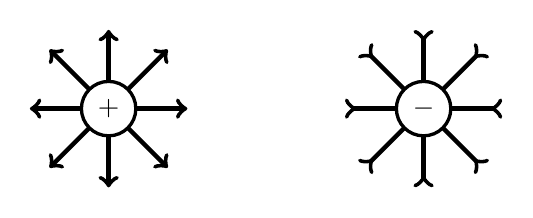
\begin{tikzpicture}[scale=2]
        \draw[<->, ultra thick](-0.5,0)--(0.5,0);
        \draw[>-<, ultra thick](1.5,0)--(2.5,0);

        \draw[<->, ultra thick](0,-0.5)--(0,0.5);
        \draw[>-<, ultra thick](2,-0.5)--(2,0.5);

        \draw[<->, ultra thick](-0.375,-0.375)--(0.375,0.375);
        \draw[<->, ultra thick](0.375,-0.375)--(-0.375,0.375);

        \draw[>-<, ultra thick](1.625,-0.375)--(2.375,0.375);
        \draw[>-<, ultra thick](2.375,-0.375)--(1.625,0.375);

        \node[sum](+)at(0,0){$+$};
        \node[sum](-)at(2,0){$-$};
    \end{tikzpicture}
\end{center}


In generale una forza elettrica è effetto dall'interazione di una carica $q$ con un campo elettrico $\vec{E}$, indipendentemente da ciò che genera il campo elettrico. Nel 
caso di una carica stazionaria o in moto rettilineo uniforme, si considera un campo elettro-stazionario, per cui la forza generata si esprime come il prodotto per la carica 
ed il campo elettrico: 
\begin{equation}
    \vec{F}=q\vec{E}
\end{equation}

L'unità di misura fondamentale usata per analizzare fenomeni elettrici nel SI è l'Ampere $A$, intensità di corrente, che ha sostituito il Coulomb $C$, unità di carica, 
entrambe sono cognomi di scienziati che hanno studiato l'elettricità, a differenza delle restanti grandezze fondamentali. Ciò spiega come non fosse chiaramanete 
idefntificabile la causa dei fenomeni elettrici in passato. 


In caso sia presente più di una carica stazionaria nel vuoto, per determinare il campo elettrico in un dato punto si considera il principio di sovrapposizione degli effetti 
(P.S.E.), applicabile solo in situazioni di tipo lineare, come nel vuoto essendo un elemento lineare. Per il principio della sovrapposizione degli effetti, il campo in un 
punto è dato dalla somma vettoriale di tutti i campi in quel punto, per cui i campi agiscono indipendentemente l'uno dall'altro. In una configurazione a due cariche, una 
positiva ed una negativa, il campo totale agente su una carica positiva posta in una posizione $P$ risulta essere: $\vec{E}_P=\vec{E}_1+\vec{E}_2$. 
\begin{center}
    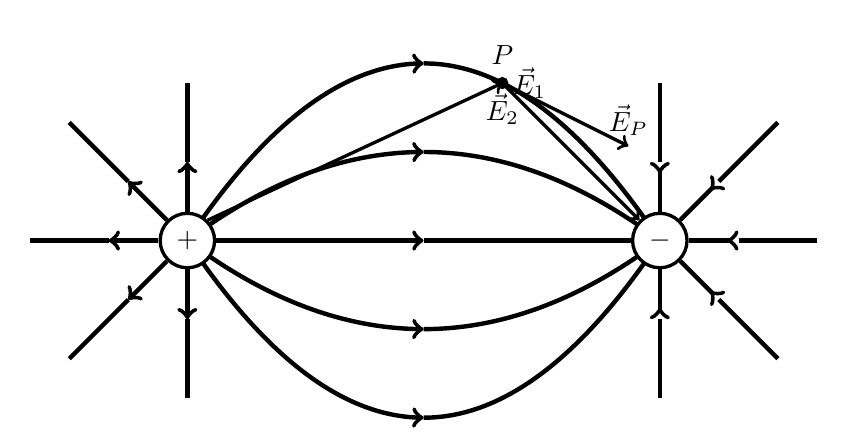
\begin{tikzpicture}[scale=2]
        \draw[->,ultra thick]plot[smooth, domain=0:1.5](\x,{0.25*(\x)*(\x-3)});
        \draw[-,ultra thick]plot[smooth, domain=1.5:3](\x,{(0.25*\x)*(\x-3)});

        \draw[->,ultra thick]plot[smooth, domain=0:1.5](\x,{-0.25*(\x)*(\x-3)});
        \draw[-,ultra thick]plot[smooth, domain=1.5:3](\x,{-0.25*(\x)*(\x-3)});

        \draw[->,ultra thick]plot[smooth, domain=0:1.5](\x,{0.5*(\x)*(\x-3)});
        \draw[-,ultra thick]plot[smooth, domain=1.5:3](\x,{(0.5*\x)*(\x-3)});

        \draw[->,ultra thick]plot[smooth, domain=0:1.5](\x,{-0.5*(\x)*(\x-3)});
        \draw[-,ultra thick]plot[smooth, domain=1.5:3](\x,{-0.5*(\x)*(\x-3)});

        \draw[<->,ultra thick](0,-0.5)--(0,0.5);
        \draw[ultra thick](0,-0.5)--(0,-1);
        \draw[ultra thick](0,0.5)--(0,1);

        \draw[>-<,ultra thick](3,-0.5)--(3,0.5);
        \draw[ultra thick](3,-0.5)--(3,-1);
        \draw[ultra thick](3,0.5)--(3,1);        

        \node[sum](+)at(0,0){$+$};
        \node[sum](-)at(3,0){$-$};

        \filldraw[circle](2,1)node[above]{$P$}circle(1pt);
        \draw[->,very thick](+.45)--(2,1)node[below]{$\vec{E}_2$};
        \draw[->,very thick](2,1)node[right]{$\vec{E}_1$}--(-.135);
        \draw[->,very thick](2,1)--(2.8,0.6)node[above]{$\vec{E}_P$};

        \draw[->, ultra thick](+.0)--(1.5,0);
        \draw[-,ultra thick](1.5,0)--(-.180);

        \draw[->,ultra thick](+.180)--(-0.5,0);
        \draw[ultra thick](-0.5,0)--(-1,0);
        \draw[-<,ultra thick](-.0)--(3.5,0);
        \draw[ultra thick](3.5,0)--(4,0);

        \draw[->,ultra thick](+.135)--(-0.375,0.375);
        \draw[->,ultra thick](+.225)--(-0.375,-0.375);
        \draw[-,ultra thick](-0.375,0.375)--(-0.75,0.75);
        \draw[-,ultra thick](-0.375,-0.375)--(-0.75,-0.75);

        \draw[-<,ultra thick](-.45)--(3.375,0.375);
        \draw[-<,ultra thick](-.315)--(3.375,-0.375);
        \draw[-,ultra thick](3.375,0.375)--(3.75,0.75);
        \draw[-,ultra thick](3.375,-0.375)--(3.75,-0.75);
    \end{tikzpicture}
\end{center}


Il campo elettrico stazionario, come il campo gravitazionale, è conservativo, per cui il lavoro svolto equivale all'opposto della differenza di energia potenziale. Per 
convenzione lo stato di riferimento dell'energia potenziale elettrica si trova ad una distanza infinita dalla carica, per cui l'energia corrisponde al lavoro necessario per 
spostare una carica $q$ da una distanza infinita ad una distanza finita $R$ da un campo elettrico $\vec{E}$. Si considera una campo elettrico generato da una carica puntiforme 
$Q$:
\begin{gather*}
    \Delta U(r)=-L=-\displaystyle\int_{+\infty}^R\vec{F}\cdot d\vec{r}\\
    \displaystyle\int_{+\infty}^Rq\vec{E}\cdot d\vec{r}=\int_{+\infty}^R\frac{1}{4\pi\varepsilon_0}\frac{qQ}{r^2}\cancelto{1}{\hat{r}\cdot \hat{r}}dr\\
    \cancelto{0}{-\displaystyle\frac{1}{4\pi\varepsilon_0}\frac{qQ}{+\infty}}+\frac{1}{4\pi\varepsilon_0}\frac{qQ}{R}
\end{gather*}
\begin{equation}
    U(r)=\frac{1}{4\pi\varepsilon_0}\frac{qQ}{R}=-L(r)
\end{equation}


Viene definito il potenziale elettrico $V$ il lavoro per unità di carica, viene misurato nel SI in Volt $V$:
\begin{equation}
    \Delta V=\displaystyle-\frac{L}{q}=-\int\frac{\vec{F}}{q}\cdot d\vec{r}=-\int\vec{E}\cdot d\vec{r}
\end{equation}
Corrisponde ad un integrale di linea del campo elettrico $\vec{E}$. 
Per un campo elettrico stazionario generato da una carica puntiforme $Q$ corrisponde a:
\begin{equation}
    V=\displaystyle\frac{1}{4\pi\varepsilon_0}\frac{Q}{R}\:\left[V\right]=\left[\frac{mN}{C}\right]
\end{equation}

In forma differenziale, il potenziale elettrico corrisponde a:
\begin{equation*}
    dV=-\vec{E}\cdot d\vec{r}=-(E_xdx+E_ydy+E_zdz)
\end{equation*}
Il differenziale $dV$ è un differenziale totale di un campo scalare $V(x,y,z)$, per cui corrisponde alla somma delle variazioni su ogni coordinata del differenziale della stessa: 
\begin{equation*}
    dV=\displaystyle\frac{\partial V}{\partial x}dx+\frac{\partial V}{\partial y}dy+\frac{\partial V}{\partial z}dz
\end{equation*}
Per il principio di indentità dei polinomi risulta:
\begin{equation*}
    \displaystyle\frac{\partial V}{\partial x}=-E_x,\:\frac{\partial V}{\partial y}=-E_y,\:\frac{\partial V}{\partial z}=-E_z
\end{equation*}

Si considera l'operatore differenziale vettoriale nabla: 
\begin{equation*}
    {\nabla}:=\left(\displaystyle\frac{\partial}{\partial x},\,\frac{\partial}{\partial y},\,\frac{\partial}{\partial z}\right)
\end{equation*}
Per cui è possibile esprimere la relazione tra il potenziale elettrico ed il campo elettrico considerando l'operazione di gradiente su un campo scalare $\vec{\nabla}V$: 
\begin{equation}
    \vec{E}=-{\nabla}V
\end{equation}
La capacità di un campo di ammettere un potenziale è una condizione sufficiente della conservatività di un campo vettoriale. Un'altra condizione sufficiente dipende dal 
risultato della circuitazione del campo, ovvero l'integrale di linea su un qualsiasi percorso chiuso $\lambda$ del campo $\vec{E}$. Se la circuitazione del campo è nulla, 
allora il campo in questione è conservativo:
\begin{equation}
    \Gamma_\lambda(\vec{E})=\displaystyle\oint_{\lambda}\vec{E}\cdot d\vec{\lambda}=0
\end{equation}
Se il campo non è conservativo, implica che il campo è variabile per cui la circuitazione risulta diversa da zero. 


Oltre all'operazione di gradiente su un campo scalare, se si considera un campo vettoriale $\vec{a}(x,y,z)$, si possono definire altre due operazioni: la divergenza ed il 
rotore. La divergenze è definita come il prodotto scalare tra l'operatore nabla ed il campo $\vec{a}$:
\begin{gather*}
    {\nabla}\cdot\vec{a}=\displaystyle\left(\frac{\partial}{\partial x}\hat{x}+\frac{\partial}{\partial y}\hat{y}+\frac{\partial}{\partial z}\hat z\right)\cdot\left(a_x\hat{x}+a_y\hat{y}+a_z\hat{z}\right)\\
    \displaystyle\frac{\partial a_x}{\partial x}\cancelto{1}{\hat{x}\cdot\hat{x}}+\frac{\partial a_y}{\partial x}\cancelto{0}{\hat{y}\cdot\hat{x}}+\frac{\partial a_z}{\partial x}\cancelto{0}{\hat{z}\cdot\hat{x}}+
    \frac{\partial a_x}{\partial y}\cancelto{0}{\hat{x}\cdot\hat{y}}+\frac{\partial a_y}{\partial y}\cancelto{1}{\hat{y}\cdot\hat{y}}+\frac{\partial a_z}{\partial y}\cancelto{0}{\hat{z}\cdot\hat{y}}+
    \frac{\partial a_x}{\partial z}\cancelto{0}{\hat{x}\cdot\hat{z}}+\frac{\partial a_y}{\partial z}\cancelto{0}{\hat{y}\cdot\hat{z}}+\frac{\partial a_z}{\partial z}\cancelto{1}{\hat{z}\cdot\hat{z}}
\end{gather*}
\begin{equation}
    {\nabla}\cdot\vec{a}=\displaystyle\frac{\partial a_x}{\partial x}+\frac{\partial a_y}{\partial y}+\frac{\partial a_z}{\partial z}
\end{equation}
Il rotore è definito come il prodotto vettoriale tra l'operatore nabla ed il campo $\vec{a}$:
\begin{gather*}
    {\nabla}\times\vec{a}=
    \begin{vmatrix}
        \hat{x} & \hat{y} & \hat{z} \\
        \displaystyle\frac{\partial}{\partial x} & \displaystyle\frac{\partial}{\partial y} & \displaystyle\frac{\partial}{\partial z}\\
        a_x & a_y & a_z
    \end{vmatrix}=
    \begin{vmatrix}
        \displaystyle\frac{\partial}{\partial y} & \displaystyle\frac{\partial }{\partial z}\\
        a_y & a_z
    \end{vmatrix}\hat{x}-
    \begin{vmatrix}
        \displaystyle\frac{\partial}{\partial x} & \displaystyle\frac{\partial}{\partial z}\\
        a_x & a_z
    \end{vmatrix}\hat{y}+
    \begin{vmatrix}
        \displaystyle\frac{\partial}{\partial x} & \displaystyle\frac{\partial}{\partial y}\\
        a_x & a_y
    \end{vmatrix}\hat{z}
\end{gather*}
\begin{equation}
    {\nabla}\times\vec{a}=\left(\displaystyle\frac{\partial a_z}{\partial y}-\frac{\partial a_y}{\partial z}\right)\hat{x}-\left(\frac{\partial a_x}{\partial z}-\frac{\partial a_z}{\partial x}\right)\hat{y}+\left(\frac{\partial a_y}{\partial x}-\frac{\partial a_x}{\partial y}\right)\hat{z}
\end{equation}

\subsubsection{Teorema di Gauss}

\begin{quotation}
    Il flusso totale, entrane o uscente, del campo elettrico $\vec{E}$ generato da cariche interne ad una qualsiasi superficie chiusa $S$, attraverso 
    la stessa superficie equivale al rapporto tra la carica totale e la costante di permettività dielettrica nel vuoto $\varepsilon_0$:
    \begin{equation}
        \Phi_{S}(\vec{E})=\displaystyle\frac{Q}{\varepsilon_0}
    \end{equation}
\end{quotation}


Analogamente alla portata di un liquido attraverso una superficie, il flusso $\Phi$ di un campo vettoriale $\vec{v}$ determina l'intensità del campo attraverso una data superficie $S$. 
\begin{center}
    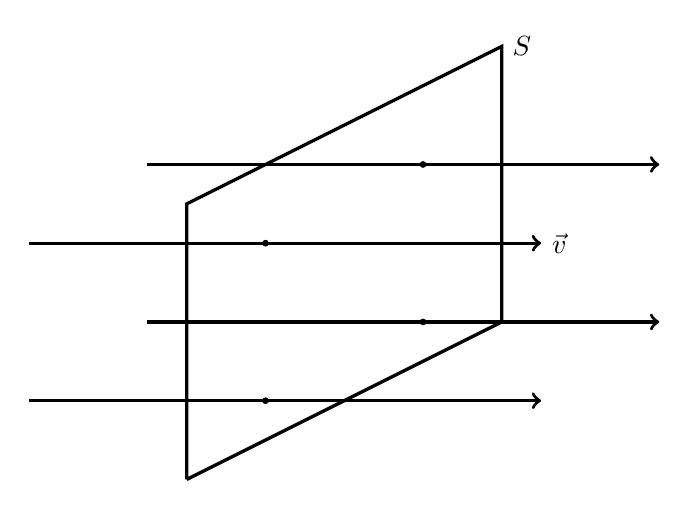
\begin{tikzpicture}[scale=2]
        \draw[very thick](0,0)--(0,1.75)--(2,2.75)node[right]{$S$}--(2,1)--(0,0);
        
        \draw[->,very thick](-1,0.5)--(2.25,0.5);
        \draw[->,very thick](-0.25,1)--(3,1);
        \draw[->,very thick](-1,1.5)--(2.25,1.5)node[right]{$\vec{v}$};
        \draw[->,very thick](-0.25,2)--(3,2);

        \filldraw[black](0.5,0.5)circle(0.5pt);
        \filldraw[black](1.5,1)circle(0.5pt);
        \filldraw[black](0.5,1.5)circle(0.5pt);
        \filldraw[black](1.5,2)circle(0.5pt);
    \end{tikzpicture}
\end{center}
Il flusso è massimo quando il campo e la superficie sono tra di loro perpendicolari: $\Phi_S(\vec{v})=|\vec{v}|\cdot S$. Per determinare il flusso attraverso una superfecie $S$ 
inclinata rispetto al campo $\vec{v}$ bisogna considerare la componente del campo che passa perpendicolarmente attraverso la superficie, per cui si definisce il versore 
giuntura di una superficie $\hat{n}_S$ come il vettore di modulo unitario, direzione normale alla superficie nel punto e di verso uscente se la superficie è concava, ed 
entrante se è convessa: $\Phi_S(\vec{v})=\vec{v}\cdot\hat{n}S$. 
In caso la superficie sia ondulata, la giacitura cambierebbe in base alla sua posizione, per cui per determinarne il flusso si considera un'approssimazione tramite la somma 
di flussi dello stesso campo attraverso suddivisioni della superficie, ognuna con una giacitura diversa: 
$\Phi_S(\vec{v})\approx\sum_{i=1}^N\vec{v}\cdot\hat{n}_iS_i$. Al diminuire della superficie $S_i$, la precisione aumenta, per cui per una superficie infinitesima si può 
determinare esattamente l'infinitesimo di flusso attraverso l'intera superficie: $\Phi_{dS}(\vec{v})=\vec{v}\cdot\hat{n}dS=d\Phi_{S}(\vec{v})$. In caso le suddivisioni 
siano finite, il flusso viene calcolato tramite una sommatoria, altrimenti per suddivisioni infinite si considera un integrale chiuso sulla superficie totale $S$:
\begin{equation}
    \displaystyle\Phi_S(\vec{v})=\int_{S}\vec{v}\cdot\hat{n}dS
\end{equation}




Nel caso del teorema di Gauss, si considera una situazione semplificata, dove è presenta una singola carica $Q$ nel centro di una superficie sferica $S$ di raggio $r$. 
Considerando una sezione infinitesima della superficie $dS$, il versore giacitura $\hat{n}$ risulta essere sempre parallelo al campo elettrico $\vec{E}$ generato dalla carica, 
poiché si trova nel centro della sfera. Per cui il campo elettrico passante per ogni sezione infinitesima è costante, considerando l'integrale del flusso: 
\begin{gather*}
    \Phi_S(\vec{E})=\displaystyle\oint_{S}E\cancelto{1}{\hat{r}\cdot\hat{n}}dS=\oint_S\frac{Q}{4\pi\varepsilon_0r^2}dS=\frac{Q}{4\pi\varepsilon_0r^2}\oint_SdS=\frac{Q}{4\pi\varepsilon_0r^2}4\pi r^2
\end{gather*} 
\begin{equation}
    \Phi_S(\vec{E})=\frac{Q}{\varepsilon_0}
\end{equation}
\begin{center}
    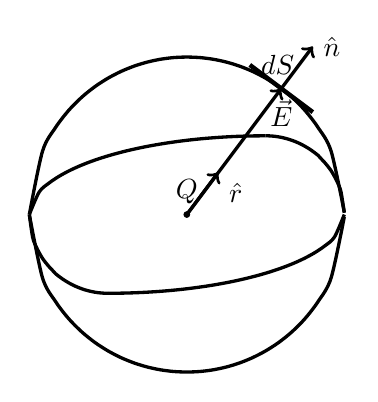
\begin{tikzpicture}[scale=2]
        \draw[-, very thick]plot[smooth, domain=-1:1](\x, {(1-(\x)^2)^0.5});
        \draw[-, very thick]plot[smooth, domain=-1:1](\x, {-(1-(\x)^2)^0.5});
        \draw[-, very thick]plot[smooth, domain=0.5:1](\x,{(0.25-(\x-0.5)^2)^0.5});
        \draw[-, very thick]plot[smooth, domain=-1:-0.5](\x,{-(0.25-(\x+0.5)^2)^0.5});
        \draw[-, very thick]plot[smooth, domain=-1:0.5](\x,{1/3*(2.25-(\x-0.5)^2)^0.5});
        \draw[-, very thick]plot[smooth, domain=-0.5:1](\x,{-1/3*(2.25-(\x+0.5)^2)^0.5});

        \filldraw[black](0,0)circle(0.5pt);

        \draw[->, very thick](0,0)node[above]{$Q$}--(0.6,0.8)node[below]{$\vec{E}$};
        \draw[->,very thick](0,0)--(0.2,0.267)node[below right]{$\hat{r}$};

        \draw[-, ultra thick](0.4,0.95)node[right]{$dS$}--(0.8,0.65);
        \draw[->,very thick](0.6,0.8)--(0.8,1.067)node[right]{$\hat{n}$};
    \end{tikzpicture}
\end{center}

Ciò implica che il campo elettrico ammette l'esistenza di sorgenti singole. Infatti se una carica si trova all'interno di una superficie chiusa, tutte le linee di campo generate 
escono attraverso la superficie, mentre se la carica si trovasse all'esterno della superficie, tutte le linee di campo entranti sarebbero necessariamente anche uscenti, ed il 
flusso totale sarebbe dato dalla somma del flusso entrante e del flusso uscente risultando nullo. 

\subsubsection{Teorema della Divergenza e I Legge di Maxwell}

Il flusso attraverso una superficie chiusa è dato dalla somma del flusso per ogni faccia della superficie. Considerando un cubo infinitesimo con faccie parallele ai piani 
cartesiani ed un campo elettrico $\vec{E}$ passante per quel cubo, si calcola il flusso totale sommando il flusso sulle sue sei faccie. 
\begin{center}
    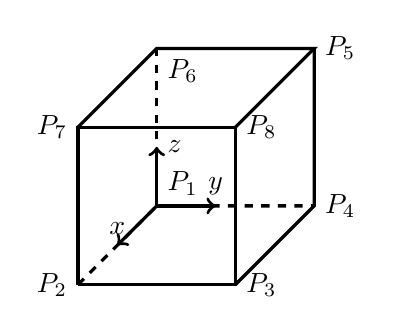
\begin{tikzpicture}[scale=2]
        \draw[-,very thick](0,0)node[left]{$P_2$}--(1,0)node[right]{$P_3$}--(1,1)node[right]{$P_8$}--(0,1)node[left]{$P_7$}--(0,0);
        \draw[dashed,very thick](0,0)--(0.5,0.5)node[above right]{$P_1$}--(1.5,0.5)node[right]{$P_4$};
        \draw[dashed,very thick](0.5,0.5)--(0.5,1.5)node[below right]{$P_6$};
        \draw[-,very thick](1,1)--(1.5,1.5)node[right]{$P_5$}--(0.5,1.5)--(0,1);
        \draw[-,very thick](1,0)--(1.5,0.5)--(1.5,1.5);
        \draw[->,very thick](0.5,0.5)--(0.25,0.25)node[above]{$x$};
        \draw[->,very thick](0.5,0.5)--(0.875,0.5)node[above]{$y$};
        \draw[->,very thick](0.5,0.5)--(0.5,0.875)node[right]{$z$};
    \end{tikzpicture}
\end{center}
\begin{align*}
    &P_1(x,y,z) &P_5(x,y+dy,z+dz)\\
    &P_2(x+dx,y,z) &P_6(x,y,z+dz)\\
    &P_3(x+dx,y+dy,z) &P_7(x+dx,y,z+dz)\\
    &P_4(x,y+dy,z) &P_8(x+dx,y+dy,z+dz)
\end{align*}

Il flusso attraverso la faccia $P_1P_2P_3P_4$ risulta essere:
\begin{equation*}
    \Phi_1(\vec{E})=\vec{E}\cdot\hat{n}dS=(E_x\cancelto{0}{\hat{x}\cdot\hat{n}}+E_y\cancelto{0}{\hat{y}\cdot\hat{n}}+E_z\cancelto{-1}{\hat{z}\cdot\hat{n}})dS=-E_zdxdy
\end{equation*}
Poiché il campo elettrico è antiparallelo alla giuntura della superficie. 


Consdierando la faccia $P_5P_6P_7P_8$, il campo elettrico varia prima di attraversare la faccia. La variazione dipende dalla variazione lungo l'asse $z$, per cui il cambiamento 
del campo elettrico dipende dalla sua derivata parziale $\displaystyle\frac{\partial\vec{E}}{\partial z}$. Il cambiamento effettivo è dato dalla derivata parziale 
moltiplicata per lo spostamento effettuato sull'asse $z$, trattandosi di un cubo infinitesimo lo spostamento è infinitesimo $dz$. Per cui il campo che attraversa la faccia 
risulta essere:
\begin{equation*}
    \vec{E}+\displaystyle\frac{\partial \vec{E}}{\partial z}dz
\end{equation*} 
Per cui il flusso risulta essere:
\begin{equation*}
    \Phi_2=\left(E_z+\displaystyle\frac{\partial E_z}{\partial z}dz\right)dxdy
\end{equation*}

Analogamente alla prima faccia, il flusso attraverso le due faccie $P_1P_2P_6P_7$ e $P_1P_4P_5P_6$ risultano essere:
\begin{gather*}
    \Phi_3=-E_ydxdz\\
    \Phi_5=-E_xdydz
\end{gather*}
Analogamente alla seconda faccia, il campo elettrico varia prima di attraversare le faccie $P_3P_4P_5P_8$ e $P_2P_3P_7P_8$, ed il loro flusso risulta essere:
\begin{gather*}
    \Phi_4=\left(E_y+\displaystyle\frac{\partial E_y}{\partial y}dy\right)dxdz\\
    \Phi_6=\left(E_x+\displaystyle\frac{\partial E_x}{\partial x}dx\right)dydz
\end{gather*}

Il flusso totale attraverso il cubo infinitesimo risulta quindi essere:
\begin{gather*}
    \Phi=\displaystyle\sum_{i=1}^6\Phi_i\\
    \begin{matrix}
        -E_zdxdy & -E_ydxdz & -E_xdydz\\
        +\left(E_z+\displaystyle\frac{\partial E_z}{\partial z}dz\right)dxdy & +\left(E_y+\displaystyle\frac{\partial E_y}{\partial y}dy\right)dxdz & +\left(E_x+\displaystyle\frac{\partial E_x}{\partial x}dx\right)dydz
    \end{matrix}\\
    \displaystyle\frac{\partial E_z}{\partial z}dxdydz+\frac{\partial E_y}{\partial y}dxdydz+\frac{\partial E_x}{\partial x}dxdydz\\
    \Phi=\left(\displaystyle\frac{\partial E_x}{\partial x}+\frac{\partial E_y}{\partial y}+\frac{\partial E_z}{\partial z}\right)dxdydz
\end{gather*}

Si cosidera il volume del cubo infinitesimo $d\tau=dxdydz$, mentre la superficie infinitesime che racchiude il volume $dS$. Il flusso attraverso il cubo equivale alla 
divergenza del campo elettrico: 
\begin{equation*}
    \Phi_{dS}(\vec{E})={\nabla}\cdot\vec{E}d\tau=d\Phi_S(\vec{E})
\end{equation*}
Per cui è possibile determinare il flusso di un campo elettrico (stazionario) $\vec{E}$ attraverso una superficie chiusa $S$, consideranro l'integrale sul volume 
racchiuso dalla superficie $\tau$ della divergenza del campo. Ciò viene chiamato teorema della divergenza. 
\begin{equation}
    \displaystyle\oint_S\vec{E}\cdot\hat{n}dS=\int_{\tau}{\nabla}\cdot\vec{E}d\tau
\end{equation} 
Per il teroema di Gauss il flusso di un campo elettrico $\vec{E}$ attraverso una qualsiasi superficie chiusa $S$ è dato dal rapporto delle carica totale $Q$ interna alla superficie 
e la permettività dielettrica nel vuoto $\varepsilon_0$. Dato un mezzo con densità uniforme di carica $\rho_Q$, la carica totale può essere espressa come l'integrale sull'intero 
volume della densità: 
\begin{equation*}
    Q=\displaystyle\int_{\tau}\rho_Qd\tau
\end{equation*}  
Per il teorema di Gauss e per il teorema della divergenza:
\begin{gather*}
    \displaystyle\int_{\tau}{\nabla}\cdot \vec{E}d\tau=\int_{\tau}\frac{\rho_Q}{\varepsilon_0}d\tau\\
    {\nabla}\cdot\vec{E}=\displaystyle\frac{\rho_Q}{\varepsilon_0}
\end{gather*}

Viene definito vettore dello spostamento elettrico nel vuoto $\vec{D}:=\varepsilon_0\vec{E}$, per cui si può esprimere l'equazione precedente come:
\begin{equation}
    {\nabla}\cdot\vec{D}=\rho_Q\,\displaystyle\left[\frac{C}{m^3}\right]
\end{equation}
Questa è la prima legge di Maxwell in forma locale. 

\subsubsection{Teorma del Rotore}

In un campo elettrico conservativo, la circuitazione lungo un qualsiasi percorso chiuso è nulla. Poiché il campo elettrico equivale all'inverso del gradiente del 
potenziale ed il potenziale è lavoro per unità di carica di un campo conservativo, su un percorso chiuso il lavoro è nullo, quindi anche la circuitazione. Esistono invece 
campi elettrici che non producono lavoro, ma forza elettro-motrice, per cui la circuitazione su un percorso chiuso è diversa da zero. 



Considerando una superficie quadrata infinitesima attraversata da un campo elettrico $\vec{E}$, si vuole calcolare la sua circuitazione, sommando la circuitazione sui suoi 
quattro lati infinitesimi, come il prodotto scalare tra il campo elettrico e lo spostamento $d\vec{\lambda}$. Per convenzione si considera una circuitazione positiva in senso 
antiorario. 
\begin{center}
    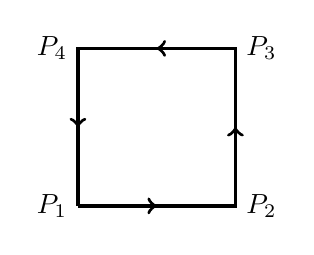
\begin{tikzpicture}[scale=2]
        \draw[-, very thick](0,0)node[left]{$P_1$}--(1,0)node[right]{$P_2$}--(1,1)node[right]{$P_3$}--(0,1)node[left]{$P_4$}--(0,0);
        \draw[->,very thick](0,0)--(0.5,0);
        \draw[->,very thick](1,0)--(1,0.5);
        \draw[->,very thick](1,1)--(0.5,1);
        \draw[->,very thick](0,1)--(0,0.5);
    \end{tikzpicture}
\end{center}
\begin{align*}
    &P_1(x,y,z)\\
    &P_2(x+dx,y,z)\\
    &P_3(x+dx,y+dy,z)\\
    &P_4(x,y+dy,z)
\end{align*}

Sul lato $P_1P_2$, il campo elettrico varia con l'aumento della coordinata $x$, poiché ogni componte del campo elettrico dipende dalle $3$ coordinate, la variazione di una 
coordinate implica una variazione di tutte le componenti del campo. La circuitazione risulta quindi essere:
\begin{equation*}
    \Gamma_1=\vec{E}\cdot d\vec{\lambda}=\left(E_x\hat{x}+\displaystyle\frac{\partial E_x}{\partial x}dx\hat{x}+E_y\hat{y}+\frac{\partial E_y}{\partial x}dy\hat{y}+E_z\hat{z}+\frac{\partial E_z}{\partial x}dz\hat{z}\right)\cdot d\vec{x}=\left(E_x+\frac{\partial E_x}{\partial x}dx\right)dx
\end{equation*}
Analogamente per il lato $P_2P_3$, il campo elettrico varia con l'aumento delle coordinata $x$ e $y$, per cui per ogni componente del campo sarà aggiunta una variazione dipendente 
dall'aumento delle $x$ e un'altra dall'aumento delle $y$:
\begin{equation*}
    \Gamma_2=\left(E_y\hat{y}+\displaystyle\frac{\partial E_y}{\partial x}dx\hat{y}+\frac{\partial E_y}{\partial y}dy\hat{y}\right)\cdot d\vec{y}=\left(E_y+\frac{\partial E_y}{\partial x}dx+\frac{\partial E_y}{\partial y}dy\right)dy
\end{equation*}

Per i lati $P_3P_4$ e $P_4P_1$ la direzione in cui vengono attraversati è opposta alla verso delle coordinate, per cui la circuitazione per questi lati è negativa:
\begin{gather*}
    \Gamma_3=-\left(E_x+\displaystyle\frac{\partial E_x}{\partial x}dx+\frac{\partial E_x}{\partial y}dy\right)dx\\
    \Gamma_4=-\left(E_y+\displaystyle\frac{\partial E_y}{\partial y}dy\right)dy
\end{gather*} 

La circuitazione totale risulta essere quindi:
\begin{gather*}
    \Gamma=\Gamma_1+\Gamma_2+\Gamma_3+\Gamma_4\\
    \begin{matrix}
        \displaystyle\left(E_x+\frac{\partial E_x}{\partial x}dx\right)dx+\left(E_y+\frac{\partial E_y}{\partial x}dx+\frac{\partial E_y}{\partial y}dy\right)dy\\
        \displaystyle-\left(E_x+\frac{\partial E_x}{\partial x}dx+\frac{\partial E_x}{\partial y}dy\right)dx-\left(E_y+\frac{\partial E_y}{\partial y}dy\right)dy
    \end{matrix}\\
    \Gamma=\left(\displaystyle\frac{\partial E_y}{\partial x}-\frac{\partial E_x}{\partial y}\right)dxdy
\end{gather*}
La circuitazione totale equivale alla componente del rotore del campo elettrico parallela alla normale al piano individuato dalla superficie descritta dal percorso $\lambda$. 
Poiché la circuitazione è uno scalare, per conservare solo questa componente si considera il prodotto scalare tra il rotore del campo elettrico ed il versore giacitura. 
Considerando il differenziale della superficie $dS=dxdy$, la circuitazione totale su una superficie infinetesimale è:
\begin{equation*}
    \Gamma_{d\lambda}=\vec{E}\cdot d\vec{\lambda}=({\nabla}\times\vec{E})\cdot \hat{n}dS=d\Gamma_\lambda
\end{equation*}
Integrando quest'ultima equazione si ottiene che la circuitazione per un qualsiasi percorso chiuso $\lambda$ di un campo elettrico (stazionario) $\vec{E}$ è esattamente il 
flusso del rotore del campo elettrico attraverso la superficie $S$ descritta dal quel percorso $\lambda$. Questo rappresenta il teorema del rotore: 
\begin{equation}
    \displaystyle\oint_{\lambda}\vec{E}\cdot d\vec{\lambda}=\int_S({\nabla}\times\vec{E})\cdot\hat{n}dS
\end{equation}

Per il teorema della circuitazione ed il teorema del rotore, per tutti i campi conservativi, il rotore di un campo elettrico è nullo, condizione necessaria affinché un campo 
vettoriale sia conservativo: 
\begin{equation}
    {\nabla}\times\vec{E}=\vec0
\end{equation}

\subsection{Corrente e Magnetismo}

La corrente è una grandezza fisica che rappresenta un flusso di cariche, convenzionalmente positive, che si muovono dentro un mezzo. Nel SI viene misurata in Ampere $A$. 
La corrente può essere definita in duo modi:  


I) Si può considerare la corrente come la somma algebrica di cariche $\Delta Q$ che passano attraverso una superficie, sezione del 
mezzo dove fluiscono, in un intervallo di tempo $\Delta Q$, ovvero la velocità in cui il flusso di cariche si muove attraverso la data superficie. Questa rappresenta solo 
un'approssimazione della corrente effettiva, viene chiamata corrente media: $i_m=\displaystyle\frac{\Delta Q}{\Delta t}$. Per ottenere la corrente effettiva, si considera il 
limite per l'intervallo di tempo di osservazione $\Delta t\to0$, in questo modo si considera la corrente istantanea, ovvero la variazione di carica istantanea:
\begin{equation}
    i:=\lim_{\Delta t\to0}\displaystyle\frac{\Delta Q}{\Delta t}=\frac{dQ}{dt}\,\left[\frac{C}{s}\right]=[A]
\end{equation}  

II) Si può formulare la corrente considerando il concetto del mezzo continuo, visione della fisica classica secondo cui il materiale è continuo. Questa visione è paradossale 
poiché a livello microscopico è stato osservato che diverse grandezze non sono continue, ma per i fini prefissati non si incontra questo paradosso. Si considera un volume 
continuo con una certa densità di carica $\rho_Q$, e in moto con una certa velocità $\vec{v}$. La corrente allora corriponde alla portata attraverso una certa superficie $S$, 
ovvero corrisponde al flusso del vettore $\rho_Q\vec{v}$ attraverso la superficie $S$: 
\begin{equation}
    i:=\displaystyle\int_S\rho_Q\vec{v}\cdot\hat{n}dS
\end{equation}

\begin{center}
    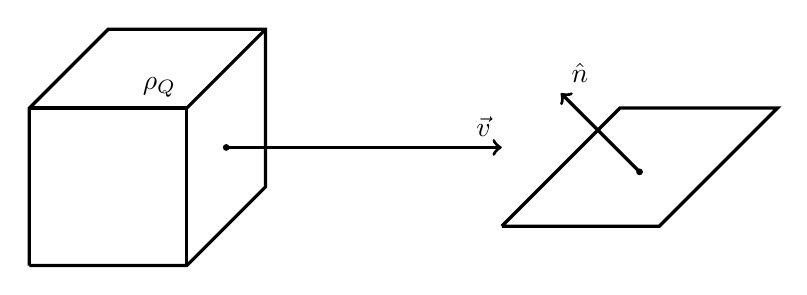
\begin{tikzpicture}[scale=2]
        \draw[-,very thick](0,0)--(1,0)--(1.5,0.5)--(1.5,1.5)--(0.5,1.5)--(0,1)--(0,0);
        \draw[-,very thick](1,0)--(1,1)node[above left]{$\rho_Q$}--(0,1);
        \draw[-,very thick](1,1)--(1.5,1.5);

        \draw[->,very thick](1.25,0.75)--(3,0.75)node[above left]{$\vec{v}$};

        \draw[-,very thick](3,0.25)--(3.75,1)--(4.75,1)--(4,0.25)--(3,0.25);
        \draw[->,very thick](3.875,0.595)--(3.375,1.095)node[above right]{$\hat{n}$};
        \filldraw[black](3.875,0.595)circle(0.5pt);
        \filldraw[black](1.25,0.75)circle(0.5pt);
    \end{tikzpicture}
\end{center}

Il vettore $\rho_Q\vec{v}$ corrisponde al vettore densità di corrente $\vec{J}\displaystyle\left[\frac{C}{m^2s}\right]$, che rappresenta la corrente in forma vettoriale. 



Come una cairca è in grado di generare un campo elettrico, una corrente è in grado di generare un campo magnetico. Nei magneti permanenti la corrente generatrice di campo 
dipende dal moviemtno degli elettroni all'interno del materiale. 

Si considera un mezzo filiforme, ovvero monodimensionale, composto di materiale conduttore, tipicamente un qualche 
metallo, dove gli elettroni sono liberi di muoversi all'interno. Si considera che un effetto esterno non definito abbia causato uno spostamento degli elettroni all'interno del filo, 
può essere dobuto all'avvicinamento di una carica negativa, spostando gli elettroni in un'altra zona del filo. Ciò crea due zone nel filo, una carica positivamente, l'altra 
carica negativamente, questa differenza di potenziale interna al filo si rappresenta come una corrente di spostamento di cariche $i$, in una certa direzione. 

Ampere ha sperimentalmente dimostrato che intorno al filo si può misurare un campo di forze, formato da linee di campo concentriche con il filo come centro. Il vero di questo 
campo si ottiene mediante la regola della mano destra: se la corrente si muove dall'alto verso il basso, allora il campo ha verso orario, altrimenti ha verso antiorario. 

\begin{center}
    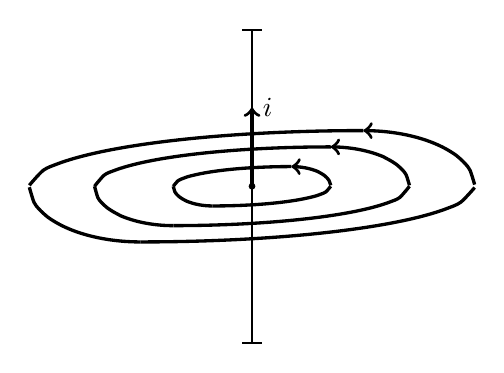
\begin{tikzpicture}[scale=2]
        \draw[<-, very thick]plot[smooth, domain=0.707:1.414](\x,{0.5*(0.5-(\x-0.707)^2)^0.5});
        \draw[-, very thick]plot[smooth, domain=-1.414:-0.707](\x,{-0.5*(0.5-(\x+0.707)^2)^0.5});
        \draw[-, very thick]plot[smooth, domain=-1.414:0.707](\x,{1/6*(4.5-(\x-0.707)^2)^0.5});
        \draw[-, very thick]plot[smooth, domain=-0.707:1.414](\x,{-1/6*(4.5-(\x+0.707)^2)^0.5});

        \draw[<-, very thick]plot[smooth, domain=0.5:1](\x,{0.5*(0.25-(\x-0.5)^2)^0.5});
        \draw[-, very thick]plot[smooth, domain=-1:-0.5](\x,{-0.5*(0.25-(\x+0.5)^2)^0.5});
        \draw[-, very thick]plot[smooth, domain=-1:0.5](\x,{1/6*(2.25-(\x-0.5)^2)^0.5});
        \draw[-, very thick]plot[smooth, domain=-0.5:1](\x,{-1/6*(2.25-(\x+0.5)^2)^0.5});

        \draw[<-, very thick]plot[smooth, domain=0.25:0.5](\x,{0.5*(0.0625-(\x-0.25)^2)^0.5});
        \draw[-, very thick]plot[smooth, domain=-0.5:-0.25](\x,{-0.5*(0.0625-(\x+0.25)^2)^0.5});
        \draw[-, very thick]plot[smooth, domain=-0.5:0.25](\x,{1/6*(0.5625-(\x-0.25)^2)^0.5});
        \draw[-, very thick]plot[smooth, domain=-0.25:0.5](\x,{-1/6*(0.5625-(\x+0.25)^2)^0.5});

        \draw[|-|, thick](0,-1)--(0,1);
        \draw[->, very thick](0,0)--(0,0.5)node[right]{$i$};
        \filldraw[black](0,0)circle(0.5pt);
    \end{tikzpicture}
\end{center}

Il campo generato dalla corrente è il campo magnetico $\vec{H}$. Le circonferenza generate sono il luogo dei punti dello spazio tangenti al campo $\vec{H}$ 
in quel punto. La circuitazione del campo $\vec{H}$ su una sua circonferenza corrisponde alla corrente concatenata $i_c$ moltiplicata per un fattore $n$, poiché potrebbero essere presenti multiple 
correnti passanti all'intrerno di quel percorso $\lambda$: 
\begin{equation*}
    \displaystyle\oint_{\lambda}\vec{H}\cdot d\vec{\lambda}=(n)i_c
\end{equation*}

Per il teorema della circuitazione:
\begin{equation*}
    \displaystyle\oint_{\lambda}\vec{H}\cdot d\vec{\lambda}=\int_S(\nabla\times\vec{H})\cdot\hat{n}dS=i_c
\end{equation*}

La corrente passante per il filo può essere espressa come il flusso della densità di carica attraverso la sezione $S'$ del materiale filiforme, questo flusso corrisponde allo 
stesso flusso per la superficie individuata dalla circonferenza $\lambda$, poiché in mezzi non metallici, ovvero conduttori, i contributi si annullano:
\begin{equation}
    \displaystyle\int_S(\nabla\times\vec{H})\cdot\hat{n}dS=\int_{S'}\vec{J}\cdot\hat{n}dS=\int_S\vec{J}\cdot\hat{n}dS
\end{equation}

\begin{center}
    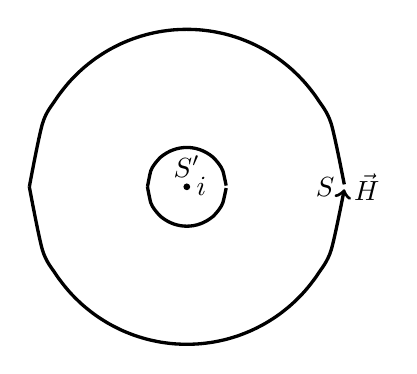
\begin{tikzpicture}[scale=2]
        \draw[-,very thick]plot[smooth, domain=-1:1](\x,{(1-(\x)^2)^0.5});
        \draw[->,very thick]plot[smooth, domain=-1:1](\x,{-(1-(\x)^2)^0.5});
        \node[right]at(1,0){$\vec{H}$};
        \node[left]at(1,0){$S$};

        \draw[-, very thick]plot[smooth, domain=-0.25:0.25](\x,{(0.0625-(\x)^2)^0.5});
        \draw[-, very thick]plot[smooth, domain=-0.25:0.25](\x,{-(0.0625-(\x)^2)^0.5});
        \node[right]at(0,0){$i$}node[above]{$S'$};
        \filldraw[black](0,0)circle(0.5pt);
    \end{tikzpicture}
\end{center}

Questa relazione tra rotore del campo magentico e vettore densità di carica viene chiamato teorema di Ampere, ed in forma locale si presenta come:
\begin{equation*}
    \nabla\times\vec{H}=\vec{J}
\end{equation*}
Considerando il vettore di induzione magnetica $\vec{B}=\mu_0\vec{H}$, dove $\mu_0$ è la costante di permabilità magnetica nel vuoto:
\begin{equation*}
    \mu_0=4\pi\cdot10^{-7}
\end{equation*}
Si esprime il teorema di Ampere in forma locale come:
\begin{equation}
    \nabla\times\vec{B}=\mu_0\vec{J}
\end{equation}
A questo risultato ottenuto da Ampere verrà aggiunto il fattore di corrente di spostamento di Maxwell. 

\subsubsection{Teorema di Ampere-Maxwell e II Legge di Maxwell}
Il teorema da Ampere da solo descrive una situazione paradossale, per cui l'intervento di Maxwell perfezionò l'analisi compiuta da Ampere. 

Per descrivere il paradosso contenuto nel teorema di Ampere si considera un filo dove scorre una certa corrente $i$. Il filo è reciso in una sezione e vengono poste due 
lamine metalliche ad ambo le parti della sezione tagliata. Maxwell osservò sperimentalmente che la corrente continuna a fluire nel resto del filo, per cui deve essere 
necessariamente presente qualcosa nella zona di vuoto tra il filo capace di muovere le cariche, per cui paradossalemente la corrente attraversa il vuoto, ma è stato descritto 
precedentemente come sia impossibile per la corrente fluire per un mezzo non conduttore come il vuoto. 

Per spiegare il paradosso, si considera che la corrente deposita sulla lamina cariche positive, mentre la corrente dall'altra parte del vuoto preleva cariche positive dalla lamina, 
quindi le due lamine sono una carica positivamente, mentre l'altra carica negativamente. La carica delle due lamine può essere spiegata per un effetto induttivo, ma fisicamente 
la corrente preleva e deposita cariche positive sulle due maglie metalliche. 


La corrente che passa attraverso il filo può essere espressa come il flusso del campo magnetico generato attraverso una cerchio di raggio $r$ e centrato nel filo:
\begin{equation*}
    i=\int_S{\vec{H}}\cdot\hat{n}dS
\end{equation*} 

Si considera inoltre un volume di base la superficie su cui si è effettuato l'operazione di flusso, che racchiude la maglia attaccata alla porzione del filo considerata. 

\begin{center}
    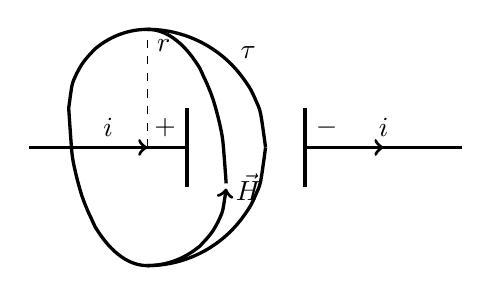
\begin{tikzpicture}[scale=2]
        \draw[-,very thick](-0.75,0)--(0.25,0)node[above left]{$+$};
        \draw[-,ultra thick](0.25,-0.25)--(0.25,0.25);
        \draw[-, very thick](1,0)node[above right]{$-$}--(2,0);
        \draw[-,ultra thick](1,-0.25)--(1,0.25);
        
        \draw[->,very thick](-0.25,0)node[above]{$i$}--(0,0);
        \draw[->,very thick](1.25,0)--(1.5,0)node[above]{$i$};
        \draw[dashed](0,0)--(0,0.75)node[below right]{$r$};

        \node[right]at(0.5,-0.25){$\vec{H}$};
        \node[above left]at(0.75,0.5){$\tau$};

        \draw[->,very thick]plot[smooth, domain=0:0.5](\x,{-0.25-(0.25-(\x)^2)^0.5});
        \draw[-,very thick]plot[smooth, domain=-0.5:0](\x,{+0.25+(0.25-(\x)^2)^0.5});
        \draw[-,very thick]plot[smooth, domain=-0.5:0](\x,{+0.25-2*(0.25-(\x)^2)^0.5});
        \draw[-,very thick]plot[smooth, domain=0:0.5](\x,{-0.25+2*(0.25-(\x)^2)^0.5});
        \draw[-,very thick]plot[smooth, domain=0:0.75](\x,{(0.5625-(\x)^2)^0.5});
        \draw[-,very thick]plot[smooth, domain=0:0.75](\x,{-(0.5625-(\x)^2)^0.5});
    \end{tikzpicture}
\end{center}

La corrente poiché è continua dovrebbe trovarsi anche tra le due armature, ma nel volume individuato il campo magnetico è nullo, per cui non è presente un flusso di cariche. 
Per spiegare questo paradosso si considera la corrente come variazione di carica per unità di tempo: $i=\displaystyle\frac{dQ}{dt}$. Sull'armatura considerata si accumulano 
cariche, percui è presenta una variazione di carica nel tempo. L'armatura carica produce quindi un campo elettrico, individuabile tramite il teorema di Gauss, considerando un 
cubo avente due faccie parallele alla lamina. Se la lamina è succifientemente estesa, il campo elettrico $\vec{E}$ generato è sempre ortogonale alle due faccie parallele 
alla lamina, e costante su tutta la superficie. Per simmetria la lamina genera due campi di modulo e direzione uguale e verso opposto:

\begin{center}
    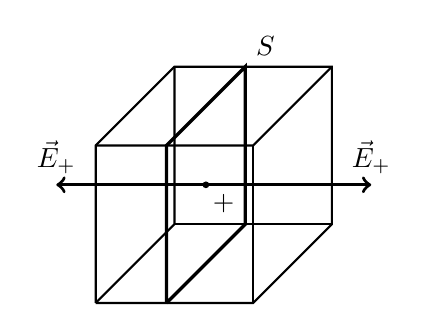
\begin{tikzpicture}[scale=2]
        \draw[-, thick](0,0)--(1,0)--(1.5,0.5)--(1.5,1.5)--(0.5,1.5)--(0,1)--(0,0);
        \draw[-, thick](0,0)--(0.5,0.5)--(0.5,1.5);
        \draw[-, thick](0.5,0.5)--(1.5,0.5);
        \draw[-, thick](0,1)--(1,1)--(1.5,1.5);
        \draw[-, thick](1,1)--(1,0);
        \draw[-,very thick](0.45,0)--(0.95,0.5)node[above left]{$+$}--(0.95,1.5)node[above right]{$S$}--(0.45,1)--(0.45,0);

        \filldraw[black](0.7,0.75)circle(0.5pt);
        \draw[->,very thick](0.7,0.75)--(1.75,0.75)node[above]{$\vec{E}_+$};
        \draw[->,very thick](0.7,0.75)--(-0.25,0.75)node[above]{$\vec{E}_+$};
    \end{tikzpicture}
\end{center}

Il flusso totale passante per la superficie chiusa $S$ corrisponde a:
\begin{equation*}
    \Phi_{S_{tot}}(\vec{E})=\displaystyle\oint_{S_{tot}}\vec{E}\cdot\hat{n}dS=\int_{2S}EdS=2ES
\end{equation*}
Per il teorema di Gauss lo stesso flusso corrisponde al rapporto tra le carica del interna alla superficie e la permettività dielettrica nel vuoto:
\begin{equation*}
    2ES=\displaystyle\frac{Q}{\varepsilon_0}
\end{equation*}

Si considera con un processo analogo anche l'armatura carica negativamente, poiché su entrambe le armature è presenta la stessa carica in modulo, i campi generati dalla due 
armature non si annulano solo nella zona tra le due, dove il campo totale è doppio. 
\begin{center}
    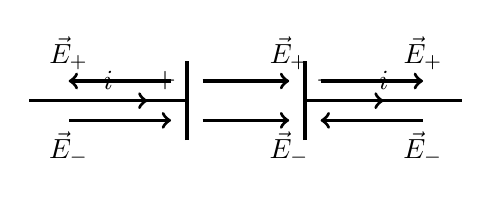
\begin{tikzpicture}[scale=2]
        \draw[-,very thick](-0.75,0)--(0.25,0)node[above left]{$+$};
        \draw[-,ultra thick](0.25,-0.25)--(0.25,0.25);
        \draw[-, very thick](1,0)node[above right]{$-$}--(2,0);
        \draw[-,ultra thick](1,-0.25)--(1,0.25);

        \draw[->,very thick](-0.25,0)node[above]{$i$}--(0,0);
        \draw[->,very thick](1.25,0)--(1.5,0)node[above]{$i$};

        \draw[->,very thick](0.35,0.125)--(0.9,0.125)node[above]{$\vec{E}_+$};
        \draw[->,very thick](1.1,0.125)--(1.75,0.125)node[above]{$\vec{E}_+$};
        \draw[->,very thick](0.15,0.125)--(-0.5,0.125)node[above]{$\vec{E}_+$};
        \draw[->,very thick](0.35,-0.125)--(0.9,-0.125)node[below]{$\vec{E}_-$};
        \draw[<-,very thick](1.1,-0.125)--(1.75,-0.125)node[below]{$\vec{E}_-$};
        \draw[<-,very thick](0.15,-0.125)--(-0.5,-0.125)node[below]{$\vec{E}_-$};
    \end{tikzpicture}
\end{center}

Si esprime la carica presente sulle armature considerando la densità superficiale di carica $\delta_Q$, per cui il campo totale (interno) generato dalle maglie risulta essere:
\begin{gather*}
    2ES=\displaystyle\frac{\delta_QS}{\varepsilon_0}\\
    E_{tot}=2E=\displaystyle\frac{\delta_Q}{\varepsilon_0}
\end{gather*}


Si esprime la quantità di carica presente sulle armature mediante la densità volumetrica di carica $\rho_Q$:
\begin{equation*}
    i=\displaystyle\frac{dQ}{dt}=\frac{d}{dt}\int_{\tau}\rho_Qd\tau
\end{equation*}
Per la prima equazione di Maxwell, e per il teorema della divergenza: 
\begin{equation*}
    i=\displaystyle\frac{d}{dt}\int_{\tau}\nabla\cdot\varepsilon_0\vec{E}d\tau=\frac{d}{dt}\oint_{S_{tot}}\varepsilon_0\vec{E}\cdot\hat{n}dS
\end{equation*}
Poiché il campo elettrico è sempre ortogonale alle armature, il flusso per l'intera superficie è uguale al flusso attraverso le sole armature $S_A$, per cui la superficie 
di integrazione diventa aperta:
\begin{equation*}
    i=\displaystyle\frac{d}{dt}\int_{S_A}\varepsilon_0\vec{E}\cdot\hat{n}dS
\end{equation*}
Poiché non si deriva per la stessa variabile di integrazione, si può invertire l'ordine delle operzaioni, considerano la derivata parziale rispetto al tempo, invece di una 
derivata totale, poiché il campo è una funzione multivariabile:
\begin{equation*}
    i=\displaystyle\int_{S_A}\varepsilon_0\frac{\partial \vec{E}}{\partial t}\cdot\hat{n}dS
\end{equation*}

Si esprime questa corrente, chiamata corrente di spostamento, mediante il flusso di un nuovo vettore di intensità di corrente $\vec{J}_S$:
\begin{equation*}
    i_S=\displaystyle\int_{S_A}\varepsilon_0\frac{\partial \vec{E}}{\partial t}\cdot\hat{n}dS=\int_{S_A}\vec{J}_S\cdot\hat{n}dS
\end{equation*}
Viene definita la corrente di spostamento di Maxwell in forma locale:
\begin{equation}
    \vec{J}_S=\displaystyle\varepsilon_0\frac{\partial \vec{E}}{\partial t}=\frac{\partial \vec{D}}{\partial t}
\end{equation}

Per la continuità delle correnti in un mezzo conduttore fluisce $\vec{J}$, mentre nel vuoto scorre $\vec{J}_S$, poiché ai due capi del filo la corrente è la stessa, necessariamente 
la corrente nel mezzo e la corrente di spostamento devono essere uguali $\vec{J}=\vec{J}_S$. Se non è presenta una variazione di campo elettrico, entrambe i vettori 
di intensità di corrente diventano nulli e non fluisce corrente nè nel filo nè nel vuoto.  

\begin{center}
    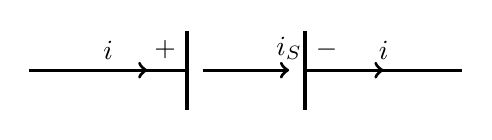
\begin{tikzpicture}[scale=2]
        \draw[-,very thick](-0.75,0)--(0.25,0)node[above left]{$+$};
        \draw[-,ultra thick](0.25,-0.25)--(0.25,0.25);
        \draw[-, very thick](1,0)node[above right]{$-$}--(2,0);
        \draw[-,ultra thick](1,-0.25)--(1,0.25);

        \draw[->,very thick](-0.25,0)node[above]{$i$}--(0,0);
        \draw[->,very thick](1.25,0)--(1.5,0)node[above]{$i$};
        \draw[->,very thick](0.35,0)--(0.9,0)node[above]{$i_S$};
    \end{tikzpicture}
\end{center}

Con aggiunta la corrente di spostamento di Maxwell, il teorema di Ampere-Maxwell, o seconda equazione di Maxwell, in forma integrale diventa:
\begin{equation*}
    \oint_{\lambda}\vec{H}\cdot d\vec{\lambda}=i_c+i_S
\end{equation*}
Per il teorema del rotore:
\begin{gather*}
    \displaystyle\oint_{\lambda}\vec{H}\cdot d\vec{\lambda}=\int_S(\nabla\times\vec{H})\cdot\hat{n}dS=i_c+i_S=\int_S(\vec{J}+\vec{J}_S)\cdot\hat{n}dS\\
    \nabla\times\vec{H}=\vec{J}+\vec{J}_S
\end{gather*}
In forma locale, si esprime mediante il rotore campo di induzione magnetica $\vec{B}$:
\begin{equation}
    \nabla\times\vec{B}=\mu_0\left(\vec{J}+\varepsilon_0\displaystyle\frac{\partial \vec{E}}{\partial t}\right)
\end{equation}

\subsection{Campo Elettro-Motore}

Il campo elettro-motore è un tipo di campo fondamentale in elettronica ed elettronica, può essere generato da conversioni energetiche, tramite induzione magnetica o un'operazione 
ibrida tra le due, come una turbina che ruota meccanicamente, insieme ad un campo magnetico per generare un campo elettro-motore che genera elettriticà. Un campo elettro-motore 
genera una differenza di potenziale o tensione, ma non è garantito che queste due grandezze coincidino. 

A differenza del campo elettrico, non è un campo conservativo: $\nabla\times\vec{E}_m\neq0$. Il lavoro per unità di carica del campo elettro-motrice, equivale alla 
forza elettro-motrice, ma non corrisponde alla grandezza fisica forza:
\begin{equation*}
    \displaystyle\int_{\lambda}\vec{E}_m\cdot d\vec{\lambda}=f.e.m.
\end{equation*}
Poiché non è un campo conservativo, cambiando il percorso $\lambda$ su cui viene spinta la carica di prova, cambierà la forza elettro-motrice generata. 



Si considera una situazione dove sono presenti due cariche a contatto, una positiva, l'altra negativa. Quando sono a contatto il campo elettro-statico complessivo generato 
dalle cariche è nullo, mentre se vengono separate mediante un campo elettro-motore $\vec{E}_m$, sarà generato anche un campo elettro-statico $\vec{E}_S$ opposto del precedente: 
$\vec{E}_m=^*-\vec{E}_S$. Questa relazione di equvialenza tra i due campi non è generale, poiché uno è un campo conservativo, mentre l'altro non conservativo. Il campo 
elettro-statico è presente solo se un campo elettro-motore ha separato le due cariche. 
La forza elettro motrice generata, per un certo percorso $\lambda$ è:
\begin{equation*}
    \displaystyle\int_{\lambda}\vec{E}_m\cdot d\vec{\lambda}=-\int_{\lambda}\vec{E}_s\cdot d\vec{\lambda}
\end{equation*}
Il percorso $\lambda$ è definito dal campo elettro-motore, la conservatività di $\vec{E}_s$ è quindi irrilevante in queste condizioni. Poiché il suo lavoro per unità di carica 
è opposto alla forza elettro motrice per un certo percorso $\lambda$, cambia anch'esso in base a questo percorso. Dato che il campo elettro-statico corrisponde all'opposto del 
gradiente del potenziale $V$, si considera solo la componente di coordinata curvilinea $\lambda$: 
\begin{equation*}
    \displaystyle\int_{\lambda}\vec{E}_m\cdot d\vec{\lambda}=\int_{\lambda}\frac{\partial V}{\partial\lambda}\cancelto{1}{\hat{\lambda}\cdot\hat{\lambda}}d\vec{\lambda}=\Delta V_{\lambda}
\end{equation*}

Quindi la forza elettro-motrice per un certo percorso $\lambda$ è uguale alla differenza di potenziale tra l'inizio e la fine del percorso creato dal campo elettro-motore. 
 


Una batteria è un oggetto che, mantenendo separate cariche positive e negative mediante reazioni chimiche all'interno, è in grado di generare una differenza di potenziale 
ed un campo elettrico-stazionario tra i due morsetti, punti di accesso di materiale conduttore, necessasari per poter usufruire della differenza di potenziale generata. 

Per misurare una differenza di potenziale si usa un volmetro, uno strumento che presenta due puntali, uno positivo ed uno negativo, resitituisce la differenza tra il potenziale 
al puntale positivo ed il puntale negativo $V_+-V_-$. Il segno della differenza di potenziale fornisce informazione sulla carica dei morsetti della batteria. Se i due morsetti 
vengono coperti con un materiale isolante come la plastica, il campo elettro-statico non ne influisce, ma il volmetro registra una tensione nulla. Per cui per misurare una 
differenza di potenziale sono necessarie delle porte di accesso di materiali conduttori, dello strumento di misura e dell'oggetto, per poter misurare il campo elettro-statico. 


Il campo elettro-statico è immagine del campo elettro-motrice con una proprietà, fino a quando non cambia il percorso. La conservatività del campo elettro-statico permette 
di esprimere il rotore del campo elettro-motore come:
\begin{equation*}
    \nabla\times\vec{E}_m=\nabla\times\vec{E}_m+\nabla\times\vec{E}_s
\end{equation*}

\subsubsection{Teorema di Faraday-Neumann-Lenz e III Legge di Maxwell}

Faraday studiò le interazioni tra il campo magnetico e la corrente. Nei suoi esperimenti usò una spira di materiale conduttore, attraversata ortogonalmente da un campo magnetico 
variabile nel tempo $\vec{H}(t)=\mu_0\vec{B}(t)$, all'interno del percorso descritto dalla spira. Faraday osservò che variando il campo magnetico, all'interno della spira 
cominciava a scorrere una corrente variabile nel tempo, ovvero un flusso di cariche. Questo flusso viene generato da un campo elettro-motore $\vec{E}_m$, indotto dal campo 
magnetico $\vec{H}(t)$. Sulla spira compare una forza elettro motrice uniformemente distribuita, poiché la corrente è uguale in ogni punto della spira. 

\begin{center}
    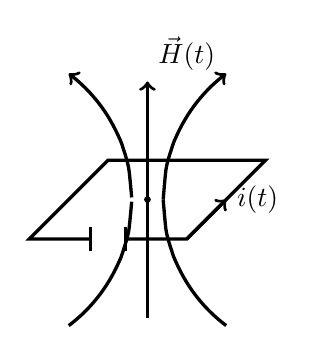
\begin{tikzpicture}[scale=2]
        \draw[|-|, very thick](-0.15,-0.25)--(0.25,-0.25)--(0.75,0.25)--(-0.25,0.25)--(-0.75,-0.25)--(-0.35,-0.25);
        \draw[->, very thick](0.25,-0.25)--(0.5,0)node[right]{$i(t)$};

        \draw[->, very thick](0,-0.75)--(0,0.75)node[above right]{$\vec{H}(t)$};
        \filldraw[black](0,0)circle(0.5pt);

        \draw[->,very thick]plot[smooth, domain=0.1:0.5](\x,{(1-(\x-1.1)^2)^0.5});
        \draw[<-,very thick]plot[smooth, domain=-0.5:-0.1](\x,{(1-(\x+1.1)^2)^0.5});
        \draw[-,very thick]plot[smooth, domain=0.1:0.5](\x,{-(1-(\x-1.1)^2)^0.5});
        \draw[-,very thick]plot[smooth, domain=-0.5:-0.1](\x,{-(1-(\x+1.1)^2)^0.5});
    \end{tikzpicture}
\end{center}

Grazie ad osservazioni sperimentali si è dimostrato che la corrente è direttamente proporzionale all'inverso della variazione del campo di induzione magnetica: 
$i(t)\propto\vec{B}(t)$, per cui si oppone al cambiamento del campo. Questo effetto venne formalizzato da Faraday, Neumann e Lenz, per esprimere la corrente generata 
si considera la circuitazione del campo elettrico indotto. Spesso si taglia il filo per indicare la differenza di potenziale descritta dalla circuitazione, rimasta invariata, 
quindi il percorso attraversato è aperto: 
\begin{equation*}
    \displaystyle\int_{\lambda}\vec{E}\cdot d\vec{\lambda}=-\frac{d\Phi(\vec{B})}{dt}=-\int_S\frac{\partial \vec{B}}{\partial t}\cdot\hat{n}dS
\end{equation*}
Dove $S$ rappresenta qualsiasi superficie con cui si concatena il campo $\vec{B}$ individuata dal percorso $\lambda$. Per il teorema del rotore:
\begin{equation}
    \displaystyle\int_S(\nabla\times\vec{E})\cdot\hat{n}dS=-\int_S\frac{\partial \vec{B}}{\partial t}\cdot\hat{n}dS
\end{equation}
In forma locale si presenta come:
\begin{equation*}
    \nabla\times\vec{E}=\displaystyle-\frac{\partial \vec{B}}{\partial t}
\end{equation*}
Poiché si parla di rotore, si può esprimere il campo elettrico come la somma del campo elettro-motore indotto e del campo elettro-statico tra la differenza di potenziale, 
anche se la loro somma è nulla, dato che il campo elettro-statio è irrotazionale:
\begin{equation}
    \nabla\times\vec{E}_m+\nabla\times\vec{E}_s=-\displaystyle\frac{\partial \vec{B}}{\partial t}
\end{equation} 
Quest'equazione rappresenta la terza legge di Maxwell. 

\subsubsection{IV Legge di Maxwell}

Rispetto ad un campo elettrico, un campo magnetico, generato da un magnete permanente o indotto da una corrente, presenta delle differenza considerevoli. Considerando un 
magnete permanetne, si definiscono nord e sud magentico le zone di comportamento del materiale, non è presenta una divisione netta tra le due zone poiché questo comportamento 
dpende da andamenenti microscopici. Il nord magnetico è la zona del mezzo dove escono linee di forza, mentre il 
sud magnetico è la zona del materiale dove entrano linee di forza. Queste linee di forza si propagano nel mezzo, senza interruzione di continuità:

\begin{center}
    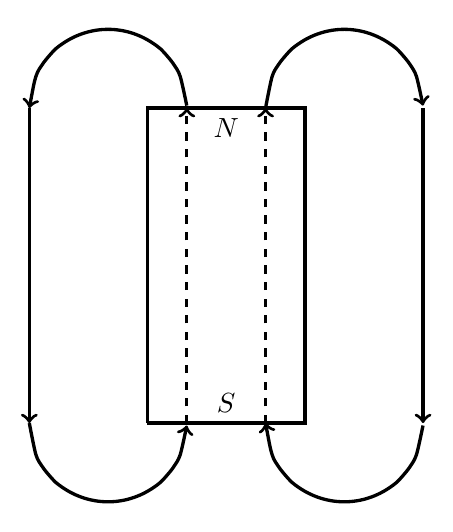
\begin{tikzpicture}[scale=2]
        \draw[-,very thick](0,0)--(0.5,0)node[above]{$S$}--(1,0)--(1,2)--(0.5,2)node[below]{$N$}--(0,2)--(0,0);

        \draw[->,very thick]plot[smooth, domain=0.75:1.75](\x,{2+(0.25-(\x-1.25)^2)^0.5});
        \draw[<-,very thick]plot[smooth, domain=-0.75:0.25](\x,{2+(0.25-(\x+0.25)^2)^0.5});
        \draw[<-,very thick]plot[smooth, domain=0.75:1.75](\x,{-(0.25-(\x-1.25)^2)^0.5});
        \draw[->,very thick]plot[smooth, domain=-0.75:0.25](\x,{-(0.25-(\x+0.25)^2)^0.5});

        \draw[->,dashed,very thick](0.25,0)--(0.25,1)--(0.25,2);
        \draw[->,dashed,very thick](0.75,0)--(0.75,1)--(0.75,2);

        \draw[->, very thick](1.75,2)--(1.75,1)--(1.75,0);
        \draw[->, very thick](-0.75,2)--(-0.75,1)--(-0.75,0);
        
    \end{tikzpicture}
\end{center}

Di conseguenza, per ogni superficie chiusa attraversata da un campo magnetico, il numero delle linee di forza entrante è pari al numero delle linee di forza uscenti, quindi 
il flusso del campo del campo magnetico $\vec{B}$ è nullo. Per il teorema della divergenza si può esprimere come:

\begin{equation}
    \displaystyle\oint_{S}\vec{B}\cdot\hat{n}dS=\int_{\tau}\nabla\cdot\vec{B}d\tau=0
\end{equation}

Di conseguenza non può esistere un monoplo magnetico, a differenza del campo elettrico, le cui sorgenti possono esistere singolarmente. Un campo la cui divergenza è nulla 
viene chiamato campo solenoidale. In forma locale si esprime la quarta ed ultima equazione di Maxwell:
\begin{equation}
    \nabla\cdot\vec{B}=0
\end{equation}

\subsection{Equazioni di Maxwell e Grandezze Fisiche}

Vengono riportata in forma locale le quattro equazioni di Maxwell, precedentemente ricavate:
\begin{equation*}
    \begin{cases}
        \nabla\times\vec{E}=-\displaystyle\frac{\partial \vec{B}}{\partial t}\\
        \nabla\times\vec{B}=\mu_0\left(\vec{J}+\displaystyle\frac{\partial \vec{D}}{\partial t}\right)\\
        \nabla\cdot\vec{D}=\rho_Q\\
        \nabla\cdot\vec{B}=0
    \end{cases}
\end{equation*}
Possono anche essere espresse in forma integrale, oppure considerando i campi di spostamento elettrico nel vuoto $\vec{D}=\varepsilon_0\vec{E}$ e di induzione magnetica nel 
vuoto $\vec{B}=\mu_0\vec{H}$. Non sempre questi campi si trovano nel vuoto, per cui si definiscono le costanti di permettività dielttrica relativa al mezzo $\varepsilon_r>1$ 
e di perambilità magnetica relativa al mezzo $\mu_r>1$. Quando vengono usate le costanti di perambilità e permettività per un mezzo diverso dal vuoto si considera $\varepsilon=\varepsilon_0\cdot\varepsilon_r$ 
e $\mu=\mu_0\cdot\mu_r$. Maggiore è la costante dielettrica relativa, più il materiale si dice dielettrico. 

Per determinare le grandezze fisiche dei campi analizzati, si considera la circuitazione del campo magnetico:
\begin{gather*}
    \displaystyle\oint_{\lambda}\vec{H}\cdot d\vec{\lambda}=i_c\to[H]=\displaystyle\frac{A}{m}
\end{gather*}
Per cui risulta che il campo magnetico si misura in Ampere per 
metro, si considera Ampere-spire, quando la corrente è concatenata più volte per la presenza di spiere sovrapposte tra di loro. Il rotore del campo magnetico $\vec{H}$ 
corrisponde ad una derivata spaziale, per cui si misura in Ampere su metro quadro:
\begin{equation*}
    [\nabla\times\vec{H}]=\displaystyle\frac{A}{m^2}
\end{equation*}

Per definire il vettore di induzione magnetica $\vec{B}$ si considera la terza equazione di Maxwell in forma integrale:
\begin{equation*}
    \displaystyle\left[\oint_{\lambda}\vec{E}\cdot d\vec\lambda=-\frac{d\Phi_S(\vec{B})}{dt}\right]\to\frac{N\cdot m}{A\cdot s}=\frac{[B]\cdot m^2}{s}\to[B]=\frac{N}{A\cdot m}:=T
\end{equation*}
Viene definita la grandezza fisica Tesla $T$ per quantificare l'intensità del campo di induzione magnetica $\vec{B}$. Ora è possibile definire la grandezza della permeabilità 
magnetica:
\begin{equation*}
    \displaystyle\left[\mu_0=\frac{{B}}{{H}}\right]\to\frac{N}{A\cdot m}\cdot\frac{m}{A}=\frac{N}{A^2}:=\frac{H}{m}
\end{equation*}
Viene definita la grandezza Henry $H$ come Newton per metro su Ampere quadro, servirà in seguito a quantificare l'auto e mutua induttanza. 

Un vettore di intensità di corrente $\vec{J}$ può esistere solo in un mezzo conduttivo, rappresenta l'unico elemento riferito al mezzo nelle equazioni di Maxwell. La corrente 
si muove nello stesso verso del vettore $\vec{J}$, ma trattandosi di uno scalare non fornisce informazioni aggiuntive sulla grandezza, poiché la direzione di una corrente è 
solo una convenzione, e le sue proprietà non cambierebbo se fluisse nel verso opposto. Una corrente si misura con un amperometro montato in serie su di un circuito, la freccia 
della corrente indica solamente la direzione dell'amperometro. Inoltre il verso della corrente indica una differenza di potenziale, dal potenziale più basso a quello 
più alto. All'interno di un materiale conduttore le cariche non si muovono spontanemanete, per cui affinché sia presente una differenza di potenziale $\Delta V=v$, deve essere 
presenta un campo elettro-statico $\vec{E}$, dovuto ad un campo elettro-motore $\vec{E}_m$. La direzione verso il potenziale più basso, ovvero il minimo del campo scalare 
potenziale è individuato dal gradiende $\nabla V$. Il gradiente è un vettore che indica il punto di minimo, per cui la direzione del vettore densità di corrente $\vec{J}$ 
dipende dall'opposto del gradiente del potenziale, ovvero dal campo elettrico: $\vec{J}\propto-\nabla V\propto=\vec{E}$. 

\begin{center}
    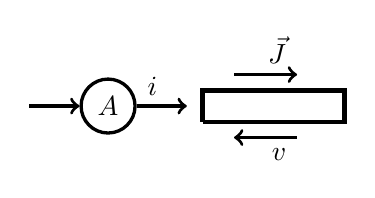
\begin{tikzpicture}[scale=2]
        \node[sum](sum)at(0,0){$A$};
        \draw[->,very thick](-0.5,0)--(sum.180);
        \draw[->, very thick](sum.0)node[above right]{$i$}--(0.5,0);
   
        \draw[-,ultra thick](0.6,-0.1)--(0.6,0.1)--(1.5,0.1)--(1.5,-0.1)--(0.6,-0.1);
        \draw[->,very thick](0.8,0.2)--(1.2,0.2)node[above left]{$\vec{J}$};
        \draw[<-,very thick](0.8,-0.2)--(1.2,-0.2)node[below left]{$v$};
    \end{tikzpicture}
\end{center}

Per i materiali di corrente, il campo elettrico impresso è uguale alla vettore di intensità di corrente moltiplicato per un fattore $\rho_e$, chiamato resistività elettrica, 
relativo al materiale considerato, chiamato resistività elettrica. Poiché il materiale internamente impedisce ad alcune cariche di fluire, per cui rallenta la nube elettronica 
che scorre nel mezzo, viene definita la grandezza fisica ohm $\Omega$ per misurare questa resistività:
\begin{equation*}
    \displaystyle\left[\vec{E}=\rho_{e}\vec{J}\right]\to\frac{N}{A\cdot s}\frac{m^2}{A}=\frac{N\cdot m^2}{A^2\cdot s}:=\Omega\cdot m
\end{equation*}
La presenza della resistività rappresenta la maggiore differenza tra lo studio dei campi e lo studio dei circuiti.  

\subsection{Onde Elettro-Magnetiche}
All'interno delle equazioni di Maxwell sono presenti dei componenti incrociati del campo elettrico $\vec{E}$ e del campo magnetico $\vec{B}$, per cui descrivono un fenomeno 
che si autosostiene, ovvero si propaga. Per determinare in che modo questo campo elettro-magnetico si propaga nello spazio, si considerano le necessarie ipotesi per poter 
descrivere semplicemente le sue proprietà. Da notare che le proprietà di questo campo si mantengono anche senza le ipotesi che considereremo. Per ottenere queste proprietà 
è sufficiente considerare solo le equazioni del rotore di Maxwell. Si studia la situazione nel vuoto, senza la presenza di conduttori, per cui la corrente di conduzione $\vec{J}$ 
è nulla e la densità di carica $\rho_Q$ è nulla: 
\begin{equation*}
    \begin{cases}
        \nabla\times\vec{E}=-\displaystyle\frac{\partial \vec{B}}{\partial t}\\
        \nabla\times\vec{B}=\mu_0\varepsilon_0\displaystyle\frac{\partial \vec{E}}{\partial t}
    \end{cases}
\end{equation*}

Per ipotesi il campo elettrico è presente solo sulla coordinata $x$ e la variazione del campo elettrico sulle $x$ rispetto alla coordinata $z$ è nulla. Le ulteriori ipotesi 
verrano discusse solo quando saranno rilevanti:
\begin{align*}
    &1)\vec{E}(x,y,z,t)=E_x(x,y,z,t)\hat{x}\\
    &2)\displaystyle\frac{\partial E_x}{\partial z}=0
\end{align*}

Dalla prima ipotesi segue che il rotore del campo elettrico ha un'unica componente $z$, per cui, per il principio di indentità dei polinomi e per la terza l'equazione di Maxwell, 
anche il campo magnetico $\vec{B}$ varia solo sulla coordinata $z$: 
\begin{gather*}
    \nabla\times\vec{E}=
    \begin{vmatrix}
        \hat{x} &\hat{y}&\hat{z}\\
        \displaystyle\frac{\partial}{\partial x}&\displaystyle\frac{\partial}{\partial y}&\displaystyle\frac{\partial}{\partial z}\\
        E_x&0&0
    \end{vmatrix}=
    \displaystyle\cancelto{0}{\frac{\partial E_x}{\partial y}}\hat{y}-\frac{\partial E_x}{\partial y}\hat{z}=-\frac{\partial \vec{B}}{\partial t}\\
    \displaystyle\frac{\partial B_x}{\partial t}=\frac{\partial B_y}{\partial t}=0\\
    \displaystyle\frac{\partial E_x}{\partial y}=\frac{\partial B_z}{\partial t}
\end{gather*}

Per la seconda equazione di Maxwell, considerando solo la componente $x$ del rotore, sempre per il principio di identità dei polinomi si ottiene:
\begin{gather*}
    \nabla\times\vec{B}=\mu_0\varepsilon_0\displaystyle\frac{\partial E_x}{\partial t}\hat{x}\\
    \left(\displaystyle\frac{\partial B_z}{\partial y}-\frac{\partial B_y}{\partial z}\right)=\mu_0\varepsilon_0\frac{\partial E_x}{\partial t}
\end{gather*}
Si definiscono due funzioni con versori diversi ortogonali, poiché non colloquiano tra di loro. 

Si mettano a sistema i risultati ottenuti:
\begin{equation*}
    \begin{cases}
        \displaystyle\frac{\partial E_x}{\partial y}=\frac{\partial B_z}{\partial t}\\
        \displaystyle\frac{\partial B_z}{\partial y}-\frac{\partial B_y}{\partial z}=\mu_0\varepsilon_0\frac{\partial E_x}{\partial t}
    \end{cases}
\end{equation*}
Si deriva rispetto al tempo la seconda equazione e invertendo l'ordine di derivazione si ottiene:
\begin{gather*}
    \displaystyle\frac{\partial^2B_z}{\partial y\partial t}-\frac{\partial^2B_y}{\partial z\partial t}=\mu_0\varepsilon_0\frac{\partial^2E_z}{\partial t^2}\\
    \displaystyle\frac{\partial}{\partial y}\frac{\partial B_z}{\partial t}-\frac{\partial}{\partial z}\cancelto{0}{\frac{\partial B_y}{\partial t}}=\mu_0\varepsilon_0\frac{\partial^2E_x}{\partial t^2}\\
    \displaystyle\frac{\partial^2E_x}{\partial y^2}=\mu_0\varepsilon_0\frac{\partial^2E_x}{\partial t^2}
\end{gather*}
Quest'equazione ottenuta descrive il comportamento di un'onda. Per ipotesi l'onda si propaga solo sulla coordinata $y$, e si considera sempre per ipotesi solamente l'onda 
diretta e si esclude quella riflessa. Le soluzioni di questo tipo di equazione d'onda sono tutte le possibili funzioni, che presentano come argomento le coordinate su cui 
l'onda si propaga, in questo caso $y$. Come argomento della soluzione si considera la traslazione dell'onda nello spazio e si inserisce il fattore correttivo $ct$, dove 
$c$ è la velocità di propagazione dell'onga:
\begin{equation*}
    Sol:=\{f(y-ct)+g(y+ct):t\geq0\}
\end{equation*}  
Per ipotesi si esclude la funzione riflessa $g$. Si sceglie la funzione più semplice come soluzione dell'onda diretta, una funzione sinusoidale. Non si può considerare $y-ct$ 
come argomento della funzione sinusoidale, poiché l'argomento deve essere monodimensionale. Si considera la relazione tra l'argomento $\alpha$, misurato in radianti e la 
variabile $y$, in metri. Viene defintia $\lambda$ lunghezza d'onda, e rappresenta la distanza tra due punti uguali dell'onda: 
\begin{equation*}
    \displaystyle\frac{y}{\alpha}=\frac{\lambda}{2\pi}\to\alpha=\frac{2\pi y}{\lambda}
\end{equation*}
Questo valore viene chimato numero d'onda. Si considera l'ampiezza massima $E_{max}$, per cui il campo elettrico si esprime come:
\begin{equation}
    E_x=E_{max}sin\left(\displaystyle\frac{2\pi (y-ct)}{\lambda}\right)
\end{equation}

Inserendo questa funzione d'onda nell'equazione d'onda precedentemente si ottiene:
\begin{gather*}
    \displaystyle\frac{\partial^2}{\partial y^2}\left(E_{max}sin\left(\displaystyle\frac{2\pi (y-ct)}{\lambda}\right)\right)=\mu_0\varepsilon_0\frac{\partial^2}{\partial t^2}\left(E_{max}sin\left(\displaystyle\frac{2\pi (y-ct)}{\lambda}\right)\right)\\
    \displaystyle E_{max}\frac{4\pi^2}{\lambda^2}sin\left(\frac{2\pi (y-ct)}{\lambda}\right)=\mu_0\varepsilon_0E_{max}\frac{4\pi^2c^2}{\lambda^2}sin\left(\frac{2\pi (y-ct)}{\lambda}\right)\\
    1=\mu_0\varepsilon_0c^2
\end{gather*}
\begin{equation}
    c=\displaystyle\frac{1}{\sqrt{\mu_0\varepsilon_0}}
\end{equation}
La velocità di propagazione dell'onda elettro-magnetica nel vuoto, corrisponde alla velocità della luce nel vuoto. Questa velocità sarà sempre minore se il campo attraversa 
un mezzo diverso dal vuoto, a causa delle costanti di permettività e permeabilità relative, per cui la velocità appena ottenuta rappresenta la massima velocità raggiungibile 
da questo tipo di onde. 

\begin{center}
    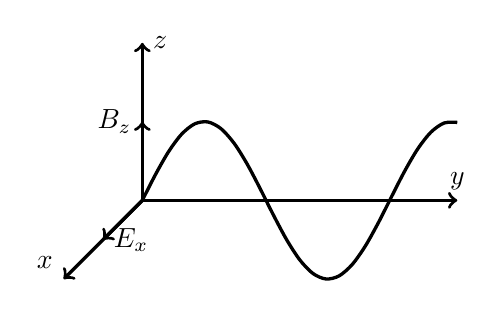
\begin{tikzpicture}[scale=2]
        \draw[->,very thick](0,0)--(2,0)node[above]{$y$};
        \draw[->,very thick](0,0)--(0,1)node[right]{$z$};
        \draw[->,very thick](0,0)--(-0.5,-0.5)node[above left]{$x$};

        \draw[->,very thick](0,0)--(0,0.5)node[left]{$B_z$};
        \draw[->,very thick](0,0)--(-0.25,-0.25)node[right]{$E_x$};
        \draw[-,very thick]plot[smooth, domain=0:2](\x,{0.5*sin(4*\x r)});
    \end{tikzpicture}
\end{center}

\subsection{Energia e Potenza}

Si considerano diverse situazione per ricavare l'energia e la potenza del campo elettrico e magnetico.

Dato un materiale condutore, si esprime la forza elettrica come la carica $q$ traspostata che interagisce con un certo campo elettrico $\vec{E}$, per cui si può esprimere 
la potenza come:
\begin{equation*}
    P=\vec{F}\cdot\vec{u}=q\vec{E}\cdot\vec{u}=\rho_Q\tau\vec{E}\cdot\vec{u}
\end{equation*}
Per un materiale conduttore il vettore intensità di carica corrisponde a $\vec{J}=\rho_Q\vec{u}$, per cui la potenza in un materiale conduttore si ricava tramite:
\begin{equation*}
    P=\tau\vec{E}\cdot\vec{J}
\end{equation*}
Si definisce la densità di potenza $P_\tau$ come la potenza $P$ generata in un certo volume $\tau$: 
\begin{equation}
    P_{\tau}=\displaystyle\frac{P}{\tau}=\vec{E}\cdot\vec{J}\,\left[\frac{W}{m^2}\right]
\end{equation}


Dato un materiale dielettrico nel continuo, dotato di una certa densità di carica $\rho_Q$. Per ricavare l'energia prodatta dal campo elettrico, si considera l'integrale 
di linea, poiché potrebbe essere presente un campo elettro-motore non conservativo, su un tratto $\lambda$ del materiale:
\begin{equation*}
    \mathscr{E}=\displaystyle\int_{\lambda}\vec{F}\cdot d\vec{\lambda}=q\int_{\lambda}\vec{E}\cdot d\vec{\lambda}
\end{equation*}

\begin{center}
    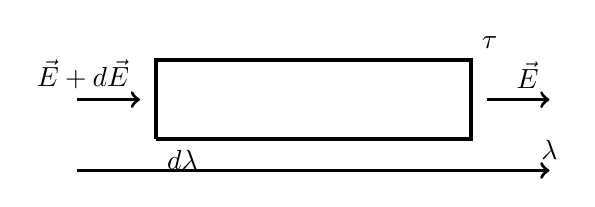
\begin{tikzpicture}[scale=2]
        \draw[-,ultra thick](0,0)node[below right]{$d\lambda$}--(2,0)--(2,0.5)node[above right]{$\tau$}--(0,0.5)--(0,0);
        \draw[->,very thick](-0.5,0.25)--(-0.1,0.25)node[above left]{$\vec{E}+d\vec{E}$};
        \draw[->,very thick](2.1,0.25)--(2.5,0.25)node[above left]{$\vec{E}$};

        \draw[->,very thick](-0.5,-0.2)--(2.5,-0.2)node[above]{$\lambda$};
    \end{tikzpicture}
\end{center}

Si considera un volumetto interno al materiale di lunghezza $d\lambda$, e si considera il campo elettrico unidirezionale, solo sulla coordinata curvilinea definita dal 
percorso $\lambda$. Per la prima equazione di Maxwell:
\begin{equation*}
    \nabla\cdot\varepsilon_0\vec{E}=\varepsilon_0\displaystyle\frac{\partial E_{\lambda}}{\partial\lambda}=\rho_Q
\end{equation*}
La carica $q$ corrisponde all'integrale della densità di carica sul volume $\tau$ del materiale considerato:
\begin{equation*}
    \mathscr{E}=\displaystyle\int_{\tau}\varepsilon_0\frac{\partial E_{\lambda}}{\partial\lambda}d\tau\cdot\int_{\lambda}\vec{E}\cdot d\vec{\lambda}
\end{equation*}
Si considera il differenziale totale dell'energia rispetto al volume $\tau$ ed alla coordinata $\lambda$:
\begin{equation*}
    d\mathscr{E}=\displaystyle\frac{\partial \mathscr{E}}{\partial \tau}d\tau+\frac{\partial\mathscr{E}}{\partial \lambda}d\lambda
\end{equation*}
Sostituendo l'integrale precedentemente ottenuto si ottiene:
\begin{gather*}
    d\mathscr{E}=d\left(\displaystyle\int_{\tau}\varepsilon_0\frac{\partial E_{\lambda}}{\partial\lambda}d\tau\cdot\int_{\lambda}\vec{E}\cdot d\vec{\lambda}\right)=\frac{\partial \mathscr{E}}{\partial \tau}d\tau+\frac{\partial\mathscr{E}}{\partial \lambda}d\lambda\\
    \displaystyle\varepsilon_0\frac{\partial E_{\lambda}}{\partial\lambda}d\tau\cdot Ed\lambda=\frac{\partial \mathscr{E}}{\partial \tau}d\tau+\frac{\partial\mathscr{E}}{\partial \lambda}d\lambda\\
    \displaystyle\frac{\partial E_{\lambda}}{\partial \lambda}d\lambda=dE\to\vec{E}\cdot d\vec{E}=EdE\\
    d\mathscr{E}=\varepsilon_0EdEd\tau\\
    \frac{d\mathscr{E}}{d\tau}=d\mathscr{E}_{\tau}=\varepsilon_0\vec{E}\cdot d\vec{E}\\
\end{gather*}
Per cui integrando entrambe le parti si ottiene la densità energetica o energia totale per unità di volume:
\begin{equation*}
    \mathscr{E}_\tau=\varepsilon_0\displaystyle\int_{0}^E\vec{E}\cdot d\vec{E}=\frac{1}{2}\varepsilon_0E^2
\end{equation*}
Si può esprimere come:
\begin{equation}
    \mathscr{E}_{\tau}=\displaystyle\frac{1}{2}\vec{E}\cdot\vec{D}\,\left[\frac{J}{m^3}\right]
\end{equation}


Dato un materiale magnetico, la densità di potenza precedentemente calcolata può essere\\espressa come:
\begin{equation*}
    P_\tau=\vec{E}\cdot\vec{J}\to dP=EJd\tau\to P=\displaystyle\int_{\tau}EJd\lambda dS=\int_{S}EdS\cdot\int_{\lambda}Jd\lambda
\end{equation*}
Si possono separare gli integrali poiché il campo elettrico dipende solo dalla superficie, mentre il vettore densità di carica dal percorso. L'integrale del campo elettrico 
su una superficie $S$ corrisponde alla differenza di potenziale $v$, mentre l'integrale dell'intensità di corrente su un percorso $\lambda$ corrisponde alla corrente passante 
in quel percorso: 
\begin{equation}
    P=v\cdot i
\end{equation}

Questa situazione avviene all'interno di un toro, un solido di forma come una ciambella, dove il campo magnetico è ortogonale al campo elettrico generato, la superficie $S$ 
è una sezione del cilindro ravvolto su sé stesso per creare il toro, dove calcolo il flusso, ed il percorso $\lambda$ è una circonferenza passante per il toro. 

La potenza si può esprimere, in questa situazione favorevole, come:
\begin{equation*}
    P=\displaystyle\frac{\partial \phi(\vec{B})}{\partial t}\oint_{\lambda}\vec{H}\cdot d\vec{\lambda}
\end{equation*}
Poiché il percorso, il campo magnetio ed il campo di induzione magnetica sono paralleli si ottiene la seguente formula:
\begin{gather*}
    P=\displaystyle\frac{dBS}{dt}H\lambda=\frac{dB}{dt}H\tau\\
    P_{\tau}=\displaystyle\frac{dB}{dt}H=\frac{d\mathscr{E}_{tot}}{dt}\\
    d\mathscr{E}_{tot}=HdB=\mu_0HdH\\
    \mathscr{E}_{tot}=\displaystyle\mu_0\int_0^HHdH=\frac{1}{2}\mu_0H^2
\end{gather*}
Questa può essere espressa come:
\begin{equation}
    \mathscr{E}=\displaystyle\frac{1}{2}\vec{H}\cdot\vec{B}
\end{equation}

\clearpage

\section{Circuiti}

Quando si studia la propagazione dei campi elettro-magnetici all'interno di materiali e circuiti, si considerano le leggi cositutive del mezzo materiale:
\begin{equation}
    \begin{cases}
        \vec{D}=\varepsilon\vec{D}\\
        \vec{B}=\mu\vec{H}\\
        \vec{J}=\sigma(\vec{E}+\vec{E}_m)+\vec{J}_m
    \end{cases}
\end{equation}
Dove $\vec{J}_m$ è la corrente indotta da un campo elettro-motore. Si ottiene quest'ultima formula, considerando la relazione tra campo elettrico e densità di corrente mediante 
resistività: $\vec{E}=\rho_e\vec{J}$. Il fattore $\sigma$ corrisponde all'inverso della resistività, per si esprime la corrente di conduzione dovuta al campo elettro-statico 
$\vec{E}$ dovuto al campo elettro-motore $\vec{E}_m$:  
\begin{gather*}
    \vec{J}=\sigma\vec{E}=\sigma(\vec{E}+\vec{E}_m)\\
\end{gather*}
Non si esclude se sia presente una corrente dovuta ad una conversione energetica, come un campo elettro-motore:
\begin{equation*}
    \vec{J}=\sigma(\vec{E}+\vec{E}_m)+\vec{J}_m
\end{equation*}
La costante $\sigma$ si può misurare in siemens $S$ per metro:
\begin{equation*}
    [\sigma]=\displaystyle\left[\frac{1}{\rho_e}\right]=\frac{1}{\Omega\cdot m}=\frac{S}{m}
\end{equation*}

Il modello circuitale viene definito tramite osservazione sperimentali, per produrre un modello matematico, con cui è possible simulare rappresentazioni fisiche non realizzabili 
o distanti dall'elettro-magnetismo. Questo modello così creato è un'approsimmazione dei fenomeni fisici in atto all'interno del circuito, ma sotto certe condizioni può 
descrivere con considerevole precisione gli andamenti del campo elettro-magnetico. 

\subsection{Principi Cardinali di Kirchoff}

I principi di Kirchoff descrivono l'andamento dell'elettro-magnetismo a regime stazionario, ovvero ogni grandezza fisica $x$ è invariante nel tempo
$\displaystyle\frac{\partial }{\partial t}x(t)=0$, ciò rappresenta una visione galileiana della fisica, per cui non descrive a pieno i fenomeni fisici. 

In questa situazione, si considerano le equazioni di Maxwell inerenti al rotore:
\begin{equation*}
    \begin{cases}
        \nabla\times\vec{E}=\vec0\\
        \nabla\times\vec{H}=\vec{J}
    \end{cases}
\end{equation*}


In forma integrale, si considera la circuitazione del campo elettrico su un qualsiasi percorso chiuso $\lambda$:
\begin{equation*}
    \displaystyle\oint_{\lambda}\vec{E}\cdot d\vec{\lambda}=0
\end{equation*}
Si separa il percorso $\lambda$ in $n$ diverse sezioni $\lambda_k$. La direzione su ogni sezione identifica sia la sezione di percorso $\lambda_k$ che il potenziale $v_k$ tra 
l'inizio e la fine del percorso $\lambda_k$. Questi potenziali vengono misurati senza mai cambiare il verso del volmetro usato. 

Il percorso chiuso $\lambda$ corrisponde all'unione di tutti i $n$ percorsi $\lambda_k$:
\begin{equation*}
    \lambda=\cup_{k=1}^n\lambda_k
\end{equation*}
Per cui la circuitazione su tutto il percorso chiuso corrisponde alla somma di ogni integrale di circuitazione su ogni sezione del percorso $\lambda$. L'integrale di circuitazione 
del campo elettrico $\vec{E}$ su un certo percorso $\lambda_k$ corrisponde all'opposto potenziale tra l'inizio e la fine del percorso:
\begin{gather*}
    -\int_{\lambda_k}\vec{E}\cdot d\vec{\lambda}=v_k\\
    \displaystyle\sum_{k=1}^n\left(-\int_{\lambda_k}\vec{E}\cdot d\vec{\lambda}\right)=\sum_{k=1}^nv_k
\end{gather*}
Poiché si trova in una situazione a regime stazionario, la circuitazione su un percorso chiuso cel campo elettrico è nullo, per cui la somma dei potenziali su ogni sezione 
del percorso chiuso è nulla:
\begin{equation}
    \displaystyle\sum_{k=1}^nv_k=0
\end{equation}
Quest'equazione si identifica come secondo principio di Kirchoff, o principio di Kirchoff alle tensioni. 
Se non si cambia mai il verso del volmetro, non sarà necessario cambiare il segno del potenziale $v_k$ nella sommatoria. Se il verso non fosse uguale per ogni potenziale, 
bisognerebbe considerare per ogni potenziale $v_k$ il suo segno nella somma algebrica. 

\begin{center}
    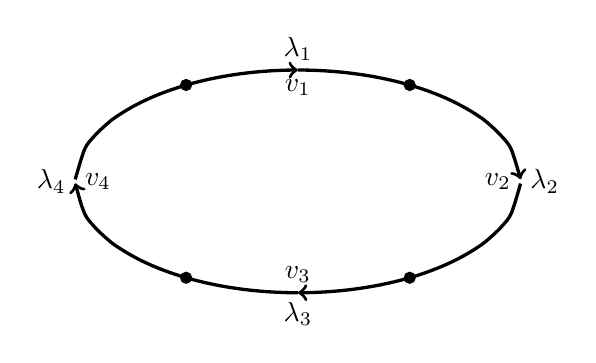
\begin{tikzpicture}[scale=2]
        \draw[->,very thick]plot[smooth, domain=0:1.414](\x,{(0.5-(1/2*\x)^2)^0.5});
        \draw[->,very thick]plot[smooth, domain=-1.414:0](\x,{(0.5-(1/2*\x)^2)^0.5});
        \draw[<-,very thick]plot[smooth, domain=0:1.414](\x,{-(0.5-(1/2*\x)^2)^0.5});
        \draw[<-,very thick]plot[smooth, domain=-1.414:0](\x,{-(0.5-(1/2*\x)^2)^0.5});


        \filldraw[black](0.71,0.612)circle(1pt);
        \node[above]at(0,0.707){$\lambda_1$};
        \node[below]at(0,0.707){$v_1$};

        \filldraw[black](0.71,-0.612)circle(1pt);
        \node[below]at(0,-0.707){$\lambda_3$};
        \node[above]at(0,-0.707){$v_3$};

        \filldraw[black](-0.71,0.612)circle(1pt);
        \node[right]at(1.414,0){$\lambda_2$};
        \node[left]at(1.414,0){$v_2$};

        \filldraw[black](-0.71,-0.612)circle(1pt);
        \node[left]at(-1.414,0){$\lambda_4$};
        \node[right]at(-1.414,0){$v_4$};
    \end{tikzpicture}
\end{center}

Per ricavare il primo principio di Kirchoff si considera la divergenza del rotore del campo magnetico $\vec{H}$:
\begin{gather*}
    \nabla\times(\nabla\times\vec{H})=\nabla\cdot\vec{J}\\
    \displaystyle\nabla\cdot\left(\displaystyle\left(\frac{\partial H_z}{\partial y}-\frac{\partial H_y}{\partial z}\right)\hat{x}-\left(\frac{\partial H_x}{\partial z}-\frac{\partial H_z}{\partial x}\right)\hat{y}+\left(\frac{\partial H_y}{\partial x}-\frac{\partial H_x}{\partial y}\right)\hat{z}\right)\\
    \displaystyle\frac{\partial^2H_z}{\partial x\partial y}-\frac{\partial^2H_y}{\partial x\partial z}-\frac{\partial^2H_x}{\partial x\partial z}+\frac{\partial^2H_z}{\partial x\partial y}+\frac{\partial^2 H_y}{\partial x\partial z}-\frac{\partial^2H_x}{\partial y\partial z}=0\\
    \nabla\cdot\vec{J}=0
\end{gather*}
Per cui la densità di corrente è solenoidale a regime stazionario. Tramite l'inverso del teorema della divergenza, si ottiene, considerando il volume $\tau$ ricoperto da una 
qualsiasi superficie chiusa $S$:
\begin{equation*}
    \displaystyle\int_{\tau}\nabla\cdot\vec{J}d\tau=\oint_{S}\vec{J}\cdot\hat{n}dS=0
\end{equation*}

Scomponendo la superficie $S$ in $n$ superfici esterne $S_k$, si può esprimere il flusso della densità di carica attravero $S$ come la somma dei flussi di $\vec{J}$ attraverso 
le superfici esterne $S_k$:
\begin{equation*}
    \displaystyle\oint_{S}\vec{J}\cdot\hat{n}dS=\sum_{k=1}^n\int_{S_k}\vec{J}\cdot\hat{n}dS=0
\end{equation*}
Il flusso della densità di corrente attraverso una superficie $S_k$ equivale alla corrente passante per quella superficie $i_k$. Poiché la somma dei flussi è nulla, allora 
necessariamente anche la somma delle correnti attraverso ogni superficie $S_k$, sezione della superficie chiusa $S$, deve essere nulla:
\begin{equation}
    \displaystyle\sum_{k=1}^ni_k=0
\end{equation}
Quest'equazione corrisponde al primo principio di Kirchoff. Una corrente può essere sia entrante che uscente in base al verso dell'amperometro, per cui sarebbe necessario 
specificarne il verso all'interno della somma algebrica. Per rappresentare il primo principio con una sommatoria semplice si misurano tutte le correnti nello stesso verso, 
per cui si esprime come la somma delle correnti entranti nella superficie chiusa $S$, alcune delle quali sono di segno negativo, corrispondenti alle correnti uscenti dalla 
superficie. 

\begin{center}
    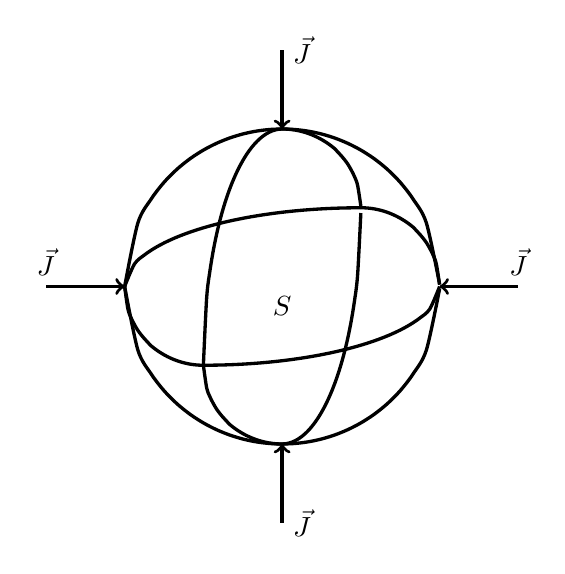
\begin{tikzpicture}[scale=2]
        \draw[-, very thick]plot[smooth, domain=-1:1](\x, {(1-(\x)^2)^0.5});
        \draw[-, very thick]plot[smooth, domain=-1:1](\x, {-(1-(\x)^2)^0.5});
        \draw[-, very thick]plot[smooth, domain=0.5:1](\x,{(0.25-(\x-0.5)^2)^0.5});
        \draw[-, very thick]plot[smooth, domain=-1:-0.5](\x,{-(0.25-(\x+0.5)^2)^0.5});
        \draw[-, very thick]plot[smooth, domain=-1:0.5](\x,{1/3*(2.25-(\x-0.5)^2)^0.5});
        \draw[-, very thick]plot[smooth, domain=-0.5:1](\x,{-1/3*(2.25-(\x+0.5)^2)^0.5});
        \draw[-, very thick]plot[smooth, domain=-0.5:0](\x,{1/2*(-1+(9-36*(\x)^2)^0.5)});
        \draw[-, very thick]plot[smooth, domain=0:0.5](\x,{1/2*(1-(9-36*(\x)^2)^0.5)});
        \draw[-,very thick]plot[smooth, domain=0:0.5](\x,{(0.25-(\x)^2)^0.5+0.5});
        \draw[-,very thick]plot[smooth, domain=-0.5:0](\x,{-(0.25-(\x)^2)^0.5-0.5});
        
        \draw[<-,very thick](0,1)--(0,1.5)node[right]{$\vec{J}$};
        \draw[<-,very thick](0,-1)--(0,-1.5)node[right]{$\vec{J}$};
        \draw[<-, very thick](1,0)--(1.5,0)node[above]{$\vec{J}$};
        \draw[<-, very thick](-1,0)--(-1.5,0)node[above]{$\vec{J}$};

        \node[below]at(0,0){$S$};
    \end{tikzpicture}
\end{center}

Queste leggi vengono anche espresse rispetto a maglie e nodi, elementi particolari, favorevoli, dei circuiti. Queste leggi inoltre possono essere usufruite dagli strumenti di 
misura. 

\subsection{Modello Circuitale a Parametri Concentrati}

Nel tempo il campo elettro-magnetico si propaga come un'onda, poiché i campi sono accoppiati nelle quattro equazioni, ma ciò non avviene a regime stazionario. Poiché le leggi di 
Kirchoff sono approssimazioni, si vuole determinare la precisione di date leggi. Si considera un canale, guida d'onda, passante per due punti $A$ e $B$. distanti $d$, 
attraversato da un flusso di cariche. Sono presenti due osservatori in $A$ e $B$, che misurano la corrente sinusoidale, entrambi aventi lo zero temporale comune. Viene 
espressa la velocità di propagazione dell'onda con $c$. Viene osservato che l'onda sinusoidale partita da $A$, viene misurata da $B$ con un certo ritardo $\tau$. 

\begin{center}
    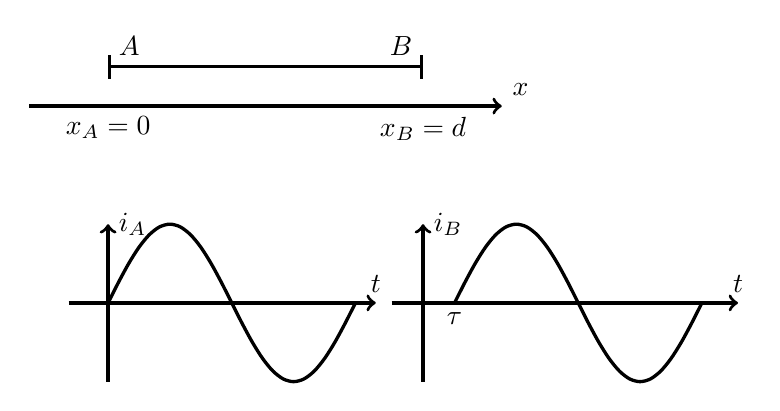
\begin{tikzpicture}[scale=2]
        \draw[|-|,very thick](0,0)node[above right]{$A$}--(2,0)node[above left]{$B$};
        \draw[->,very thick](-0.5,-0.25)--(0,-0.25)node[below]{$x_A=0$}--(2,-0.25)node[below]{$x_B=d$}--(2.5,-0.25)node[above right]{$x$};

        \draw[->,very thick](0,-2)--(0,-1)node[right]{$i_A$};
        \draw[->,very thick](-0.25,-1.5)--(1.7,-1.5)node[above]{$t$};
        \draw[-,very thick]plot[smooth, domain=0:1.57](\x,{1/2*sin(4*\x r)-1.5});

        \draw[->,very thick](2,-2)--(2,-1)node[right]{$i_B$};
        \draw[->,very thick](1.8,-1.5)--(4,-1.5)node[above]{$t$};
        \draw[-,very thick]plot[smooth, domain=2.2:3.77](\x,{1/2*sin(4*(\x-2.2) r)-1.5});
        \node[below]at(2.2,-1.5){$\tau$};
    \end{tikzpicture}
\end{center}


Si suppone che l'onda non si attenui, per cui l'ampiezza in $A$ è uguale all'ampiezza in $B$: 
\begin{equation*}
    \begin{cases}
        i_A(t)=I\sin(\omega t)\\
        i_B(t)=I\sin(\omega(t-\tau))
    \end{cases}
\end{equation*}

Poiché gli operatori interni alla funzione sinusoidale sono adimensionali, bisogna esprimere la correlazione tra l'angolo in radianti $\alpha$ e l'intervallo di tempo $t$. 
Si identifica l'intervallo di tempo in cui avviene una riproduzione completa dell'onda $T$, in radianti $2\pi$. Per cui si considera la relazione:
\begin{equation*}
    t:\alpha=T:2\pi\to\displaystyle\alpha=\frac{2\pi}{T}t
\end{equation*}
La pulsazione $T$ dell'onda sinusoidale corrisponde al fattore ${2\pi}/T$, misurato in radianti al secondo:
\begin{equation*}
    \omega=\displaystyle\frac{2\pi}{T}\,\left[\frac{\mbox{rad}}{s}\right]
\end{equation*}
Si considera un ciclo, una singola riproduzione della sinusoide. Per determinare quante volte si ripete in un intervallo di tempo si considera la grandezza fisica frequenza:
\begin{equation*}
    f=\displaystyle\frac{1}{T}
\end{equation*}
Consdierando una qualsiasi superficie chiusa che contiene il canale $AB$, la densità elettrica è prima entrante in $A$ e poi uscente in $B$, per cui la divergenza di $\vec J$ 
è nulla.


Il sistema si dice sia quasi-stazionario se il lettore $A$ legge la stessa corrente del lettore $B$, ovvero è presente un errore accettabile o trascurabile. 
Per cui le due correnti sono approsimativamente congruenti:
\begin{gather*}
    i_A\cong i_B\\
    I\sin\displaystyle\left(\frac{2\pi}{T}t\right)\cong I\sin\left(\frac{2\pi}{T}t-\frac{2\pi}{T}\tau\right)\\
    \tau=\displaystyle\frac{d}{c}\to \displaystyle 2\pi f\frac{d}{c}=2\pi d\frac{f}{c}=\frac{2\pi d}{\lambda}\\
    \tau\to 0\iff \lambda>>d
\end{gather*}
L'errore è trascurabile se la lunghezza d'onda è considerevolmente maggiore della distanza tra il trasmettitore ed il ricevitore. 
L'uso del modello adatto dipende dal valore delle grandezze trattate, in elettrotecnica si studiano frequenze nell'
ordine dei $GHz$, per cui si considerano modelli di circuiti adimensionali, nei quali, dal punto di vista euclidiano, tutti i punti coincidono. In questo modo si possono 
trattare i campi in un ambiente quasi-stazionario, quindi usando le leggi di Kirchoff; poiché ancora non disponiamo di modelli di calcolo abbastanza avanzati per poter 
descrivere sistemi elettro-magnetici molto complessi che richiedono l'uso delle equazioni di campo. 

Si può rappresentare quest'approssimazione 
nei termini dei tempi o degli spazi, oppure tramite la velocità come $c\to\infty$, per 
esplicitare l'impossibilità fisica di questa situazione, considerando la formula per la velocità di propagazione delle onde elettro-magnetiche attraverso un mezzo materiale, 
ciò si ottiene solo se il prodotto tra la permettività e la permabilità è nullo: $\mu\cdot\varepsilon=0$. In base a quale delle costanti è nulla si determinano diverse 
regioni, caratterizzate da diverse propietà fisiche. Un circuito è formato da varie regioni collegate l'una tra l'altra, come fosse un mosaico. 
La denominazione di queste regioni che ne segue è arbitraria:

\subsubsection{Regione N}
Si considera la regione nulla, una regione di vuoto circuitale, diversa dal vuoto fisico, dove le costanti di permettività e permeabilità sono entrambe nulla, per cui ci si 
trova in uno stato di quasi-stazionarietà elettro-magnetica. Inoltre la costante $\sigma$ è anch'essa nulla. In questa situazione di vuoto, le equazioni costitutive del mezzo 
assumono tutte valori nulli. Dalle equazioni di Maxwell risulta che il campo elettrico è sempre conservativo $\nabla\times\vec{E}=0$, e la densità elettrica è solenoidale $\nabla\cdot\vec{J}=0$. 
Ciò permette di scegliere arbitrariamente due punti per poter definire una differenza di potenziale. 

\begin{equation*}
    \begin{cases}
        \vec{D}=\varepsilon\vec{D}=0\\
        \vec{B}=\mu\vec{H}=0\\
        \vec{J}=\sigma(\vec{E}+\vec{E}_m)+\vec{J}_m=0
    \end{cases}
\end{equation*}

\subsubsection{Regione EQP}
Si considera il duale di una regione, una regione che presenta delle proprietà opposte rispetto ad un'altra regione. La regione di equipotenzialtità, o conduttore perfetto o 
corto circuito ideale è la regione duale della regione nulla. Presenta anch'essa la quasi-stazionarietà del campo elettro-magnetico, ma la resistività elettrica è nulla, per 
cui $\sigma\to\infty$, di conseguenza il campo elettrico è nullo $\vec{E}=0$ ed la densità di corrente impressa è nulla $\vec{J}_m=0$ La terza legge costitutiva del mezzo da luogo 
ad una forma indeterminata, per cui il valore della densità di corrente, non nullo e finito, non può essere determinato mediante le equazioni di Maxwell. Sapendo con quali 
regioni è collegata sarebbe possibile determinare la densità di corrente attraverso questa regione. Inoltre poiché il campo elettrico è nullo non può essere presenta una 
differenza di potenziale. 

\begin{equation*}
    \begin{cases}
        \vec{D}=\varepsilon\vec{D}=0\\
        \vec{B}=\mu\vec{H}=0\\
        \vec{J}=\sigma(\vec{E}+\vec{E}_m)+\vec{J}_m=\infty\cdot0\to\vec{J}=?
    \end{cases}
\end{equation*}

\subsubsection{Regione C}

Nella regione di condensatore ideale, è presente uno stato di quasi-stazionarietà magnetica $\vec{B}=0$ ed il fattore $\sigma=0$. Il campo elettro-motore è nullo $\vec{E}_m=0$ 
e la densità di corrente indotta è nulla $\vec{J}_m=0$. La permettività elettrica assume un valore non nullo. 

\begin{equation*}
    \begin{cases}
        \vec{D}=\varepsilon\vec{D}\neq0\\
        \vec{B}=\mu\vec{H}=0\\
        \vec{J}=\sigma(\vec{E}+\vec{E}_m)+\vec{J}_m=0
    \end{cases}
\end{equation*}

Per le equazioni di Maxwell si ottiene che il campo elettrio in questa regione è conservativo $\nabla\times\vec{E}=0$, e il rotore del campo magnetico dipende dal solo campo 
di spostamento elettrico $\nabla\times\vec{H}=\displaystyle\frac{\partial H}{\partial t}$. In questa regione è presente un materiale puramente dielettrico, verrà in seguito 
identificata come un condensatore, caratterizzato dalla grandezza fisica capacità $C$, il rapporto tra la carica compresa in una sezione di spazio e la differenza di potenziale 
tra l'ingresso e l'uscita del condensatore:
\begin{equation*}
    C=\displaystyle\frac{Q}{v}\,\left[\frac{A\cdot s}{V}\right]
\end{equation*}

\subsubsection{Regione LM}

La regione di induttore ideale, si trova in uno stato di quasi-stazionarietà elettrica $\varepsilon=0$, la permeabilità è non nulla, ed il valore $\sigma\to\infty$, per 
ottenere una forma indeterminata nelle leggi costitutive del mezzo. Rappresenta 
il duale del condensatore ideale. Il campo elettro-motore è nullo $\vec{E}_m=0$, la densità di corrente di induzione è nulla $\vec{J}_m=0$. Il campo elettrico $\vec{E}$ è tale 
da presentare valori finiti per densità di corrente, ma non ricavabili dalle equazioni di Maxwell, poiché si presenta in forma indeterminata nelle leggi costitutive del mezzo. 
Si ricava da Maxwell che il rotore del campo elettrico è pari al rotore del campo elettrico indotto, una particolare classe di campi elettro-motori generati all'interno di 
fenomeni elettrici, $\nabla\times\vec{E}=\nabla\times\vec{E}_i$. 
Poiché $\mu\neq0$, si ha $\nabla\times\vec{E}_i=\displaystyle-\frac{\partial B}{\partial t}$, mentre il rotore del campo magnetico è pari alla densità di corrente 
$\nabla\times\vec{H}=\vec{J}$, per cui i campi sono disaccoppiati. 

\begin{equation*}
    \begin{cases}
        \vec{D}=\varepsilon\vec{D}=0\\
        \vec{B}=\mu\vec{H}\neq0\\
        \vec{J}=\sigma(\vec{E}+\vec{E}_m)+\vec{J}_m=\infty\cdot0\to\vec{J}=?
    \end{cases}
\end{equation*}

Questa regione identifica un materiale puramente magnetico che non può condurre, ma può indurre un campo magnetico, tale regione verrà in seguito identificato con l'induttore, 
definito dalla grandezza fisica induttanza $L$. 

\subsubsection{Regione R}

Questa regione descrive il resistore ideale in uno stato di quasi-stazionarietà elettro-magnetica $\mu=0$, $\varepsilon=0$. Dove la resisività elettrica è non nulla e finita 
$\sigma\neq0$, il campo elettro-motore e la densità di corrente indotta sono entrambi nulli $\vec{E}_m=0$, $\vec{J}_m=0$.

\begin{equation*}
    \begin{cases}
        \vec{D}=\varepsilon\vec{D}=0\\
        \vec{B}=\mu\vec{H}=0\\
        \vec{J}=\sigma(\vec{E}+\vec{E}_m)+\vec{J}_m=\sigma\vec{E}
    \end{cases}
\end{equation*}

Rappresenta un materiale in cui il mezzo è resistivo puro. In questo materiale, il campo elettrico è conservativo $\nabla\times\vec{E}=0$ e la densità di corrente è solenoidale 
$\nabla\cdot\vec{J}=0$. Questa regione verrà identificata dal parametro concentrato resistenza $R$. 

\subsubsection{Regione FEM}

In questa regione, generatore ideale di forza elettro motrice, è presenta una quasi-stazionarietà elettro-magnetica $\mu=0$ e $\varepsilon=0$. La resistività elettrica è nulla, 
$\sigma\to\infty$, il campo elettro-motore è non nullo e finito, per cui è presente un campo elettro-statico $\vec{E}_s=\vec{E}_m$, poiché il campo elettrico indotto è nullo 
$\vec{E}=0$ per $\mu=0$. Mentre la densità di corrente indotta è nulla $\vec{J}_m=0$. 

\begin{equation*}
    \begin{cases}
        \vec{D}=\varepsilon\vec{D}=0\\
        \vec{B}=\mu\vec{H}=0\\
        \vec{J}=\sigma(\vec{E}+\vec{E}_m)+\vec{J}_m=\infty\cdot0\to\vec{J}=?
    \end{cases}
\end{equation*}

La regione rappresenta un materiale dove è presente una pura forza elettro-motrice $\nabla\times\vec{E}\neq0$, e la densità di corrente è solenoidale $\nabla\cdot\vec{J}$. 
Questa regione genera corrente, ma avendo conducibilità nulla, non la attraversa, invece fluisce nelle regioni collegate. 
Verrà identificata da un parametro concentrato, la tensione erogata.

\subsubsection{Region IG}

Questa regione rappresenta un generatore ideale di corrente, in uno stato di quasi-stazionarietà elettro-magnetica $\mu=0$ e $\varepsilon=0$. La resistività elettrica è infinita 
$\sigma\to\infty$, il campo elettro-motore è nullo $\vec{E}_m=0$, e la densità di corrente idotta è non nulla e definita $\vec{J}_m=0$. 

\begin{equation*}
    \begin{cases}
        \vec{D}=\varepsilon\vec{D}=0\\
        \vec{B}=\mu\vec{H}=0\\
        \vec{J}=\sigma(\vec{E}+\vec{E}_m)+\vec{J}_m=\vec{J}_m
    \end{cases}
\end{equation*}

Poiché la resistività elettrica tende ad infinito, il valore del campo elettrico $\vec{E}$ è indeterminato e non può essere ricavato mediante le equazioni di Maxwell. In 
questa situazione, il campo elettrico è conservativo $\nabla\times\vec{E}=0$ e la densità di corrente è solenoidale $\nabla\cdot\vec{J}=0$. Rappresenta un materiale in cui il mezzo genera una corrente, verrò 
in seguito identificato dal parametro concentrato corrente erogata.

\subsection{Bipolo/Multipolo e Porta/Multiporta}

Introducendo parametri concentrati è possibile ricomporre il problema della quasi-stazionarietà. 

Un bipolo viene definito come una o più regioni che colloquiano dall'esterno tra due poli. Un polo viene sempre identificato con una regione di equipotenzialtità. Poiché in 
queste regioni non è presente una differenza di potenziale, tra due di queste regioni è possibile esista $v$. In elettrotecnica si riferisce ai poli con il termine morsetti, 
rappresentano un ingresso ad una regione. Una porta viene definita come una o più regioni dove la corrente di entrata di uscita sono uguali $\nabla\cdot\vec{J}=0$.

\begin{center}
    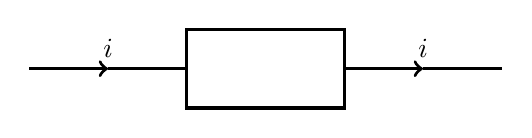
\begin{tikzpicture}[scale=2]
        \node[block](c){};
        \draw[->,very thick](-1.5,0)--(-1,0)node[above]{$i$};
        \draw[-,very thick](-1,0)--(c.180);
        \draw[->,very thick](c.0)--(1,0)node[above]{$i$};
        \draw[-,very thick](1,0)--(1.5,0);
    \end{tikzpicture}
\end{center}
Questa struttura a bipoli non è accessibile all'interno, le proprietà e le caratteristiche interne vengono definite a priori, e non possono essere ricavate dalle leggi 
dell'elettro-magnetismo. Dall'esterno si osserva solo un campo elettro-statico $\vec{E}_s$. Le informazioni note di un bipolo sono dovute ai parametri concentrati. 

Viene definito un multipolo come una o più regioni aaccessibile da una sequenza di morsetti. Viene definita multiporta un moltipolo con un numero pari di morsetti i quali 
a coppie rispettano le condizioni di una porta. 

\begin{center}
    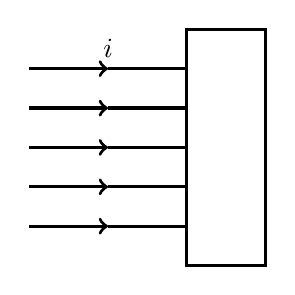
\begin{tikzpicture}[scale=2]
        \node[lblock](c)at(-0.25,0){};
        \draw[->,very thick](-1.5,0)--(-1,0);
        \draw[-,very thick](-1,0)--(-0.5,0);
        \draw[->,very thick](-1.5,0.25)--(-1,0.25);
        \draw[-,very thick](-1,0.25)--(-0.5,0.25);
        \draw[->,very thick](-1.5,0.5)--(-1,0.5);
        \draw[-,very thick](-1,0.5)node[above]{$i$}--(-0.5,0.5);
        \draw[->,very thick](-1.5,-0.25)--(-1,-0.25);
        \draw[-,very thick](-1,-0.25)--(-0.5,-0.25);
        \draw[->,very thick](-1.5,-0.5)--(-1,-0.5);
        \draw[-,very thick](-1,-0.5)--(-0.5,-0.5);
    \end{tikzpicture}
\end{center}

Per convenzione si considerano le correnti sempre entranti, ovvero si considera costante il verso dell'amperometro, per cui le correnti uscenti si indicano con il segno 
opposto. Il verso delle correnti indica solo la direzione di riferimento dell'amperometro, risptto a cui vengono misurate le correnti, che possono essere concordi, per cui 
si trovano con segno positivo, o discordi, quindi si rappresentano con segno negativo. In questo modo si possono rappresentare tutte le correnti come entranti. Per cui bisogna 
essere metodici nell'assegnazione dei segni alle grandezze fisiche misurate, poiché cambiano in base al riferimento scelto. 

\begin{center}
    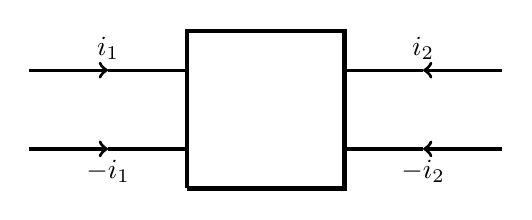
\begin{tikzpicture}[scale=2]
        \draw[-,ultra thick](-0.5,-0.5)--(-0.5,0.5)--(0.5,0.5)--(0.5,-0.5)--(-0.5,-0.5);

        \draw[->,very thick](-1.5,0.25)--(-1,0.25)node[above]{$i_1$};
        \draw[-,very thick](-1,0.25)--(-0.5,0.25);
        \draw[->,very thick](-1.5,-0.25)--(-1,-0.25)node[below]{$-i_1$};
        \draw[-,very thick](-1,-0.25)--(-0.5,-0.25);

        \draw[->,very thick](1.5,0.25)--(1,0.25)node[above]{$i_2$};
        \draw[-,very thick](1,0.25)--(0.5,0.25);
        \draw[->,very thick](1.5,-0.25)--(1,-0.25)node[below]{$-i_2$};
        \draw[-,very thick](1,-0.25)--(0.5,-0.25);
    \end{tikzpicture}
\end{center}

Dato un dipolo, si esprime il riferimento del volmetro come una freccia che indica il morsetto positivo. La differenza di potenziale si calcola come la differenza tra il 
morsetto positivo ed il morsetto negativo $v=V_+-V_-$. Si individuano due convenzioni a seconda se il verso della corrente è concorde o discorde al verso del potenziale, questi 
versi rappresentano i riferimenti usati dagli strumenti di misura. Le modalità di misura cambiano il segno all'interno delle equazioni, queste due convenzioni rappresentano 
due letture opposte della stessa situazione. 

\begin{center}
    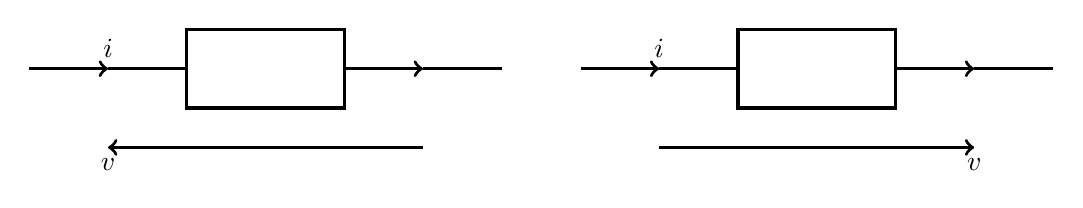
\begin{tikzpicture}[scale=2]
        \node[block](c)at(0,0){};
        \draw[->,very thick](-1.5,0)--(-1,0)node[above]{$i$};
        \draw[-,very thick](-1,0)--(c.180);
        \draw[->,very thick](c.0)--(1,0);
        \draw[-,very thick](1,0)--(1.5,0);
        \draw[->,very thick](1,-0.5)--(-1,-0.5)node[below]{$v$};

        \node[block](c1)at(3.5,0){};
        \draw[->,very thick](2,0)--(2.5,0)node[above]{$i$};
        \draw[-,very thick](2.5,0)--(c1.180);
        \draw[->,very thick](c1.0)--(4.5,0);
        \draw[-,very thick](4.5,0)--(5,0);
        \draw[<-,very thick](4.5,-0.5)node[below]{$v$}--(2.5,-0.5);
    \end{tikzpicture}
\end{center}


Se la corrente ed il potenziale hanno verso concorde si considera la convenzione dei generatori, se hanno verso discorde rappresentano la convenzione degli utilizzatori, 
queste convenzioni esprimono solamente come viene effettuata la misura. 


Nella convenzione dei generatori, la corrente di cariche positive fluisce dal potenziale più alto al potenziale più basso, per cui è il potenziale concorde che spinge le 
cariche, prodotto da un campo elettro-motore $\vec{E}_m$, quindi questa regione produce energia. Questo potenziale agisce come una forza elettro motrice, ma non può essere 
poiché in un regime di quasi-stazionarietà il campo elettrico è conservativo $\nabla\times\vec{E}=0$. 


Nella convenzione degli utilizzatori la corrente si muove di moto naturale, per cui la regione non produce ma utilizza energia elettrica prodotta da un'altra zona. Mostra 
gli effetti imposti dall'esterno sulla regione. Poiché non producono energia, non è presente un campo elettro-motore $\vec{E}_m=0$. 


Quando ci si trova in una di queste convenzioni, per determinare se il bipolo è un generatore o un utilizzatore si considera il verso della corrente e del potenziale. Se una 
di queste due grandezze è negativa, allora la situazione analizzata rappresenta l'altra convenzione. Se entrambe sono negative rappresenta comunque la convenzione, poiché 
entrambe le grandezze sono l'opposto. Per identificare se sono dei generatori o degli utilizzatori si considera la potenza $P=iv$, se i segni sono discordi la potenza è negativa 
e la situazione analizzata appartiene all'altra convenzione. 

Per cui se si analizza con una convenzione dei generatori e la potenza è positiva, si tratta di un generatore, se la potenza è negativa, si tratta di un utilizzatore. 
Analogamente per la convenzione degli utilizzatori, se la potenza è positiva, si tratta di un utilizzatore, se la potenza è negativa, si tratta di un generatore. 



Si determinano le leggi costitutive e i parametri concentrati dei bipoli. Le uniche regioni che non hanno leggi costitutive del mezzo sono il vuoto ed il suo duale l'
equipotenziale, poiché l'unico elemento in queste regioni è rispettivamente il volmetro e l'amperometro, che non influiscono sulle leggi costitutive. 

\subsubsection{Condensatore Ideale}

La regione C, viene identificata come il condensatore, una regione di quasi-stazionarietà magnetica, viene identificata come due linee parallele, collegate a morsetti. Viene 
associato al parametro concentrato capacità $C$, misurata in Farad $F$. Queste grandezze devono essere attribuite a priori, non possono essere determinate sulla base di leggi. 

\begin{center}
    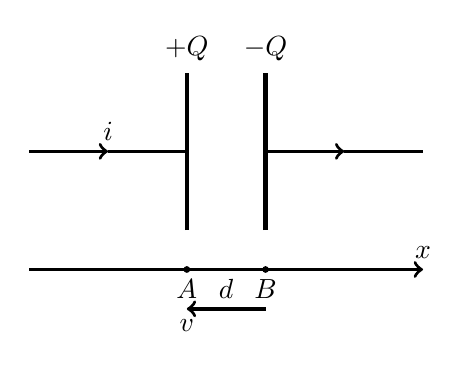
\begin{tikzpicture}[scale=2]
        \draw[->,very thick](-1.5,0)--(-1,0)node[above]{$i$};
        \draw[-,very thick](-1,0)--(-0.5,0);
        \draw[-,ultra thick](-0.5,-0.5)--(-0.5,0.5)node[above]{$+Q$};
        \draw[-,ultra thick](0,-0.5)--(0,0.5)node[above]{$-Q$};
        \draw[->,very thick](0,0)--(0.5,0);
        \draw[-,very thick](0.5,0)--(1,0);

        \draw[->,very thick](-1.5,-0.75)--(1,-0.75)node[above]{$x$};
        \filldraw[black](-0.5,-0.75)circle(0.5pt);
        \filldraw[black](0,-0.75)circle(0.5pt);
        \node[below]at(-0.5,-0.75){$A$};
        \node[below]at(0,-0.75){$B$};
        \node[below]at(-0.25,-0.75){$d$};
        \draw[->,very thick](0,-1)--(-0.5,-1)node[below]{$v$};
    \end{tikzpicture}
\end{center}

Si è analizzato precedentemente la situazione di un condensatore a faccie piane e parallele su cui si deposita una carica $+Q$ su una faccia, accumulata per un flusso di 
cariche positive $i$, e un accumulo di cariche negative $-Q$ sull'altra, poiché la stessa corrente ne sottrae cariche positive. Il campo elettrico generato tra le due 
faccie del condensatore corrisponde al rapporto tra la densità superficiale $\sigma$ delle lamine e della costante di permettività $\varepsilon$:
\begin{equation*}
    E=\displaystyle\frac{\sigma}{\varepsilon}
\end{equation*}
Le due faccie si trovano ad una distanza $d$ tra di loro, il campo elettrico è monodimensionale, poiché ha solo componenti sulla direzionee $x$. Il gradiente del potenziale 
in un caso monodimensionale corrisponde alla derivata rispetto all'unica direzione:
\begin{equation*}
    -\nabla V=-\displaystyle\frac{dV}{dx}=E_x
\end{equation*}
Si considera in forma integrale, dove i limiti di integrazione corrispondo al potenziale in $A$ ed in $B$, e le coordinate sulle $x$ dei due punti. Si considera per semplicità 
il punto $A$ cooincidente con l'origine dell'asse $x_A=0$, mentre il punto $B$ corrisponde alla distanza $x_B=d$:
\begin{equation*}
    -\displaystyle\int_{A}^BdV=\int_0^dE_xdx
\end{equation*}

Poiché si misura la densità di carica sulla piastra positiva, il campo elettrico è strettamente positivo, affinché il potenziale sia positivo si impone il volmetro come 
morsetto positivo sul punto $A$. Quindi il condensatore rappresenta un utilizzatore. Il potenziale risulta:
\begin{equation*}
    v=\displaystyle\frac{\sigma}{\varepsilon}d
\end{equation*}

Il calcolo della capacità dipende dalla geometria del singolo condensatore. Per evitare questo passagio si esprime la densità di carica $\sigma$ rispetto alla quantità 
accumulata sulla faccia positiva:
\begin{equation*}
    \sigma=\displaystyle\frac{Q}{S}\to v=\frac{QS}{\varepsilon}d
\end{equation*}
La capacità viene definita come il rapporto tra la carica positiva accumulata e la lettura positiva del volmetro:
\begin{equation}
    C:=\displaystyle\frac{Q}{v}=\varepsilon\frac{S}{d}\,[F]
\end{equation}
Si può esprimere la grandezza fisica della permittività dielettrica rispetto alla capacità:
\begin{equation*}
    [\varepsilon]=\displaystyle\frac{A\cdot s}{V\cdot m}
\end{equation*} 
Per cui per una data superficie, la carica accumulata su di essa p pari alla sua capacità per la lettura positiva del volmetro:
\begin{equation*}
    Q=Cv
\end{equation*}
In questo modo non si ottentono informazioni sulle dimensioni del circuito, ovvero la distanza tra i morsetti. Queste informazioni sono criptate all'interno della regione, 
non determinabili a posteriori. 


Vengono definiti le leggi costitutive del condensatore ideale, rappresentano le realzioni tra il potenziale e la corrente, misurate dall'esterno della regione. 
Si considera la definizione della corrente come variazione di carica nel tempo:
\begin{equation*}
    i=\displaystyle\frac{dQ}{dt}=\frac{d(Cv)}{dt}=\cancelto{0}{v\frac{dC}{dt}}+C\frac{dv}{dt}
\end{equation*}
In questo caso il parametro concentrato della capacità è tempo invariante, per cui la sua derivata è nulla. Regioni con parametri concentrati costanti si chiama tempo 
invariante. In generale non si analizzano i parametri concentrati dei generatori, ma dei bipoli passivi. Per cui, in convenzione degli utilizzatori, la legge costitutiva del 
mezzo in forma differenziale del condensatore ideale risulta essere:
\begin{equation}
    i=\displaystyle C\frac{dv}{dt}
\end{equation}
Se ci trovassimo nella convenzione dei generatori, dovremmo cambiare di segno il potenziale. In forma integrale si considerano gli intervalli di integrazione dall'inizio 
della misura per $t=0$ e alla fine della misura $t$. Il differenziale del potenziale rappresenta il differenziale di una differenza di potenziali, per cui il suo integrale rappresenta la differenza tra il potenziale alla fine della misura ed all'inizio:
\begin{equation*}
    \displaystyle\int_{v(0^-)}^{v(t)}dv=\frac{1}{C}\int_{0}^tidt
\end{equation*}
Si usa la notazione $0^-$, per comprendere il valore che assume la grandezza all'inizio esatto della misurazione, ma è nella maggior parte dei casi superfluo, poiché la funzione 
potenziale rispetto al tempo è continua quindi $v(0^-)=v(0^+)$. Si ottiene, risolvendo l'integrale:
\begin{equation*}
    v(t)=\displaystyle\int_0^tidt+v(0)
\end{equation*}
La componente integrale rappresenta l'evoluzione del potenziale al fluire della corrente all'interno del condensatore, ma risente del valore del potenziale all'inizio della misura, 
chiamato fattore di memoria. Per cui i bipoli dotati di un fattore che dipende dall'inizio della misurazione vengono chiamati bipoli con memoria, presentano o il potenziale 
o la corrente in forma differenziale. Se la memoria è nulla, si dice che il bipolo parte scarico, altrimenti si dice carico al valore assunto. In questa rappresentazione non 
sono limitati gli intervalli di tensioni possibili all'interno del condensatore, ma nella realtà non si può creare un oggetto fisico capace di avere una tensione illimiata. 

La potenza (istantanea) del condensatore ideale è come il potenziale e la corrente dipendente dal tempo:
\begin{equation*}
    P(t)=v(t)\cdot i(t)
\end{equation*}
In caso siano presenti più correnti, la potenza si ottiene considerando un morsetto di riferimento su cui si calcolano le differenze di potenziali moltiplicate per la 
corrente passante per quel morsetto. Sommando tutti queste componenti si ottiene la potenza istantanea per quel multipolo. 
Si esprime mediante la legge costitutiva del condensatore ideale in forma differenziale:
\begin{equation*}
    P=vC\displaystyle\frac{dv}{dt}
\end{equation*}
Poiché ci troviamo nella convenzione degli utilizzatori, se questa potenza fosse negativa, il condensatore erogherebbe energia elettrica. 

La potenza corrisponde alla derivata rispetto al tempo dell'energia, per cui diventa:
\begin{gather*}
    \displaystyle\frac{d\mathscr{E}}{dt}=Cv\frac{dv}{dt}\\
    d\mathscr{E}=Cvdv
\end{gather*}
Poiché questo bipolo ha memoria, la sua evoluzione nel tempo potrebbe assumere valori discordi alla memoria, fisicamente se si collega il condensatore carico ad altre regioni 
che assorbe il potenziale, questo si scarica, alimentando le regioni collegate. In quel lasso di tempo in cui alimenta un oggetto esterno il condensatore si comporta da 
generatore. Può generare tramite conversione (bipolo attivo) oppure come un bipolo passivo. La differenza tra bipolo attivo e passivo dipende dall'energia del bipolo. 
Si può esprimere l'energia del condensatore in forma integrale, definita tra due istanti di tempo. Per convenzione si considera l'inizio dell'intervallo al tempo di 
costruzione del condensatore, in termini matematici tempo remotissimo $-\infty$, dove l'energia contenuta è nulla, fino ad un certo tempo $t$. Si assume che il potenziale 
al tempo di costruzione sia nullo, per cui il condensatore è scarico quando viene costruito. 
\begin{gather*}
    \displaystyle\int_{\cancelto{0}{\mathscr{E}(-\infty)}}^{\mathscr{E}(t)}d\mathscr{E}=C\int_{\cancelto{0}{v(-\infty)}}^{v(t)}vdv\\
    \mathscr{E}(t)=C\displaystyle\frac{1}{2}v^2(t)
\end{gather*}
La capacità è definita come una grandezza positiva, per cui l'energia è strettamente positiva, ed al massimo nulla per un certo di istante di tempo $t$. Poiché l'energia 
è sempre positiva il condensatore si comporta come un bipolo passivo. Per cui il condensatore ideale è un bipolo passivo tempo invariante con memoria. 

\subsubsection{Induttore Ideale}

Il bipolo induttore ideale è il duale del condensatore ideale, presenta uno stato di quasi-stazionarietà elettrica. La dualità permette di mantenere la forma delle equazioni 
e cambiare solamente le grandezze fisiche usate. L'induttanza $L$ è il duale della capacità $C$. 
Considerando la legge costitutiva del mezzo del condensatore, si ottiene dualmente la legge costitutiva dell'induttore ideale:
\begin{equation*}
    i(t)=\displaystyle C\frac{dv(t)}{dt}\to v(t)=L\frac{di(t)}{dt}
\end{equation*}

Si vuole esprimere il duale della carica per poter esprimere il potenziale come la derivata rispetto al tempo di una certa grandezza. Il duale della carica corrisponde 
al flusso del campo magnetico, per cui la derivata rispetto al tempo di questo flusso equivale all'opposto una forza elettro motrice, ma poiché ci troviamo nella convenzione 
degli utilizzatori, si considera di segno positivo:
\begin{equation*}
    v=\displaystyle\frac{d\Phi(B)}{dt}
\end{equation*}

I parametri concentrati vengono definiti tra il rapporto di due grandezze elettro-magnetiche. Viene definito il parametro concentrato mem, rapporto tra la carica ed il flusso, 
parametro dei mem-sistori, nuovo componente dell'elettrotecnica. 

\end{document}